% $Header: /cvsroot/latex-beamer/latex-beamer/solutions/conference-talks/conference-ornate-20min.en.tex,v 1.7 2007/01/28 20:48:23 tantau Exp $

\documentclass[10pt]{beamer}

\mode<beamer>
{
  \usetheme{default}
  \usecolortheme[rgb={0,0,0.8}]{structure}
  %\setbeamercolor{normal text}{bg=blue!50}
  %\setbeamercolor{normal text}{fg=blue!50}
  % or ...

  %\setbeamercovered{transparent}
  % or whatever (possibly just delete it)
}


\usepackage[english]{babel}
% or whatever

%\usepackage[latin1]{inputenc}
% or whatever

\usepackage{times}
\usepackage[T1]{fontenc}
% Or whatever. Note that the encoding and the font should match. If T1
% does not look nice, try deleting the line with the fontenc.

%\usepackage{newcent}
%\usefonttheme{structuresmallcapsserif}

\usepackage{amssymb,latexsym,amsmath}
\usepackage{amsthm}
\DeclareMathOperator*{\argmin}{arg\,min}
\DeclareMathOperator*{\argmax}{arg\,max}

\usepackage{mathtools}
\input xy 
\xyoption{all}
\usepackage[latin1]{inputenc}
\usepackage{color}
\usepackage{tikz}
\usepackage{fontawesome}


\title[Gaussian Processes for Time Series Forecasting] % (optional, use only with long paper titles)
{Gaussian Processes for Time Series Forecasting}

%\subtitle

\author[Dr. Juan Orduz] % (optional, use only with lots of authors)
{Dr. Juan Orduz}
% - Give the names in the same order as the appear in the paper.
% - Use the \inst{?} command only if the authors have different
%   affiliation.

\institute[PyCon DE \& PyData Berlin 2019] % (optional, but mostly needed)
{

}
% - Use the \inst command only if there are several affiliations.
% - Keep it simple, no one is interested in your street address.

\date[ PyCon DE \& PyData Berlin 2019] % (optional, should be abbreviation of conference name)
{PyCon DE \& PyData Berlin 2019}
% - Either use conference name or its abbreviation.
% - Not really informative to the audience, more for people (including
%   yourself) who are reading the slides online

\subject{data science}
% This is only inserted into the PDF information catalog. Can be left
% out.



% If you have a file called "university-logo-filename.xxx", where xxx
% is a graphic format that can be processed by latex or pdflatex,
% resp., then you can add a logo as follows:

\pgfdeclareimage[height=0.7cm]{university-logo}{images/logo.png}
\logo{\pgfuseimage{university-logo}}

% If you wish to uncover everything in a step-wise fashion, uncomment
% the following command:

%\beamerdefaultoverlayspecification{<+->}


\begin{document}

\begin{frame}
  \titlepage
\end{frame}

%\begin{frame}{Contenido}
%\tableofcontents
%\end{frame}

\begin{frame}{Overview}
{{\bf Aim:} Give a better intuition on the notion of Gaussian Process Regression}
\tableofcontents
\end{frame}

\section{Introduction}

\begin{frame}{Multivariate Normal Distribution}{\cite{multivariate_normal_orduz_2019}}
$X = (X_1, \cdots, X_d)$ has a{ \bf multinormal distribution} if every linear combination is normally distributed. The joint density has the form

$$
p(x|m,K_0) =\frac{1}{\sqrt{(2\pi)^{d}|K_0|}}\exp\left(-\frac{1}{2}(x - m)^T K_0^{-1}(x - m)\right)
$$
%(2\pi)^{−d/2}|K_0|^{−1/2}\exp\left(-\frac{1}{2}(x−m)^T {K_0}^{-1}(x−m)\right)

where $m \in \mathbb{R}^d$ is the {\bf mean vector} and  $K_0 \in M_d(\mathbb{R})$ is the (symmetric, positive definite) {\bf covariance matrix}.

\begin{center}
\begin{figure}
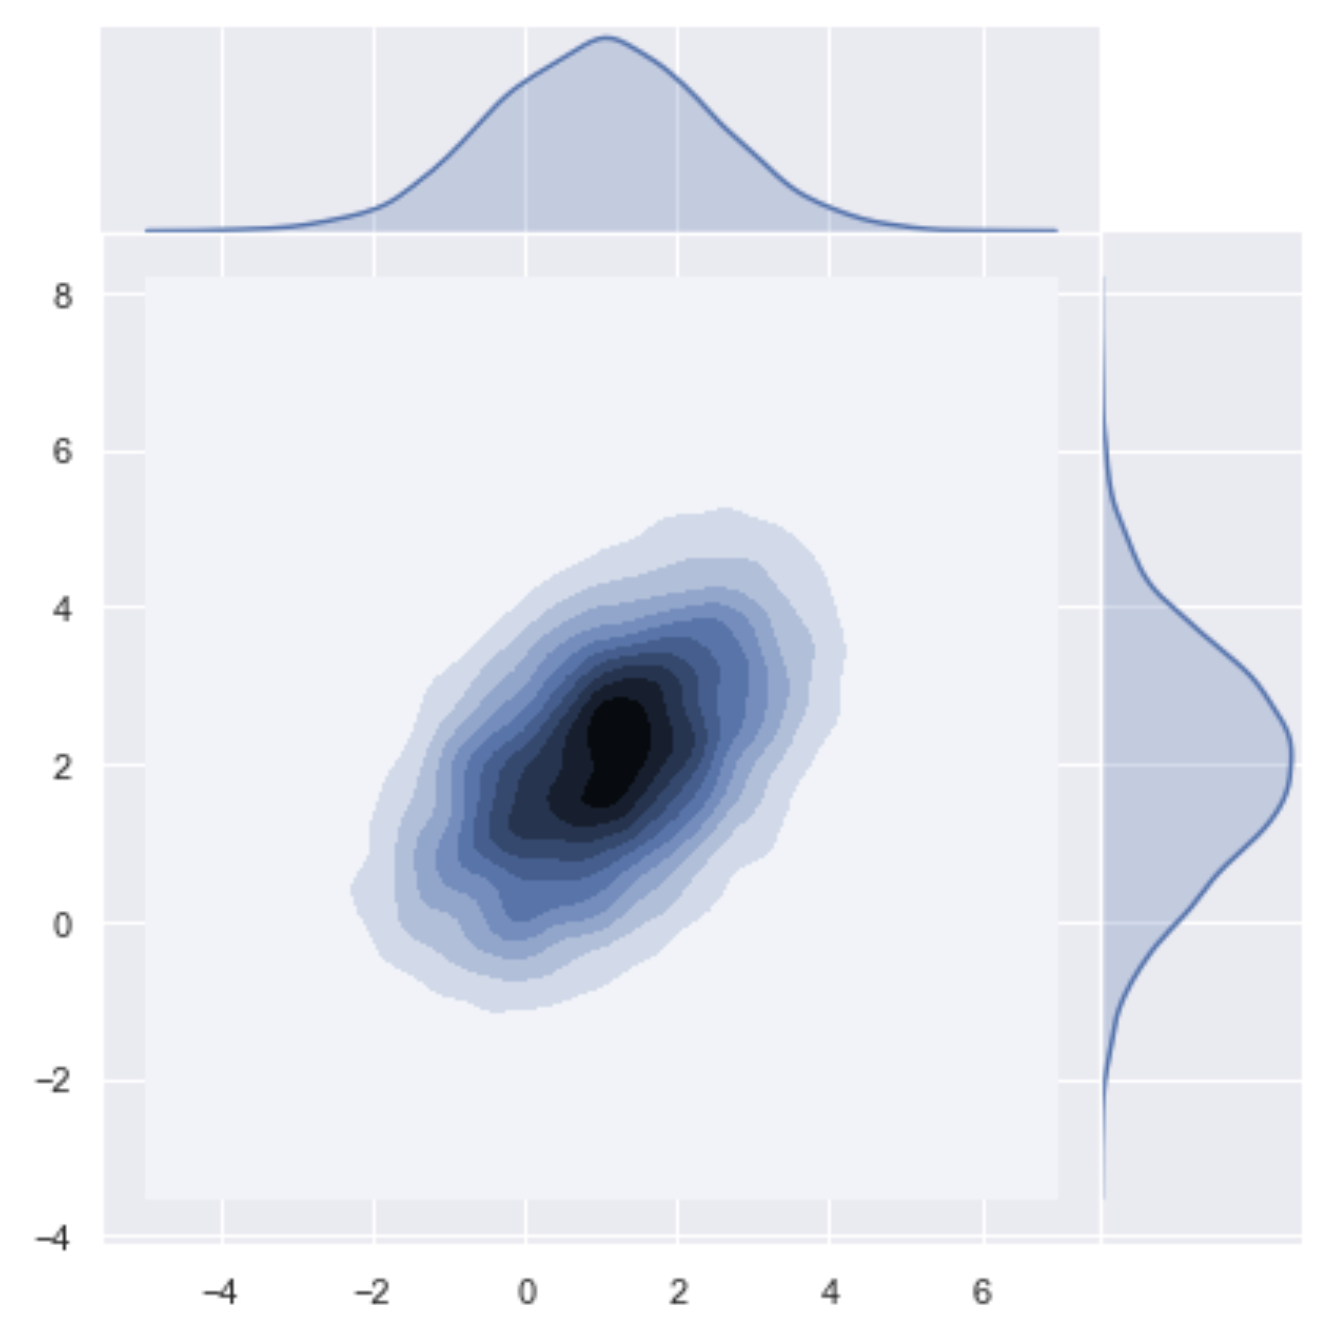
\includegraphics[scale=0.15]{images/multinormal_density.png} 
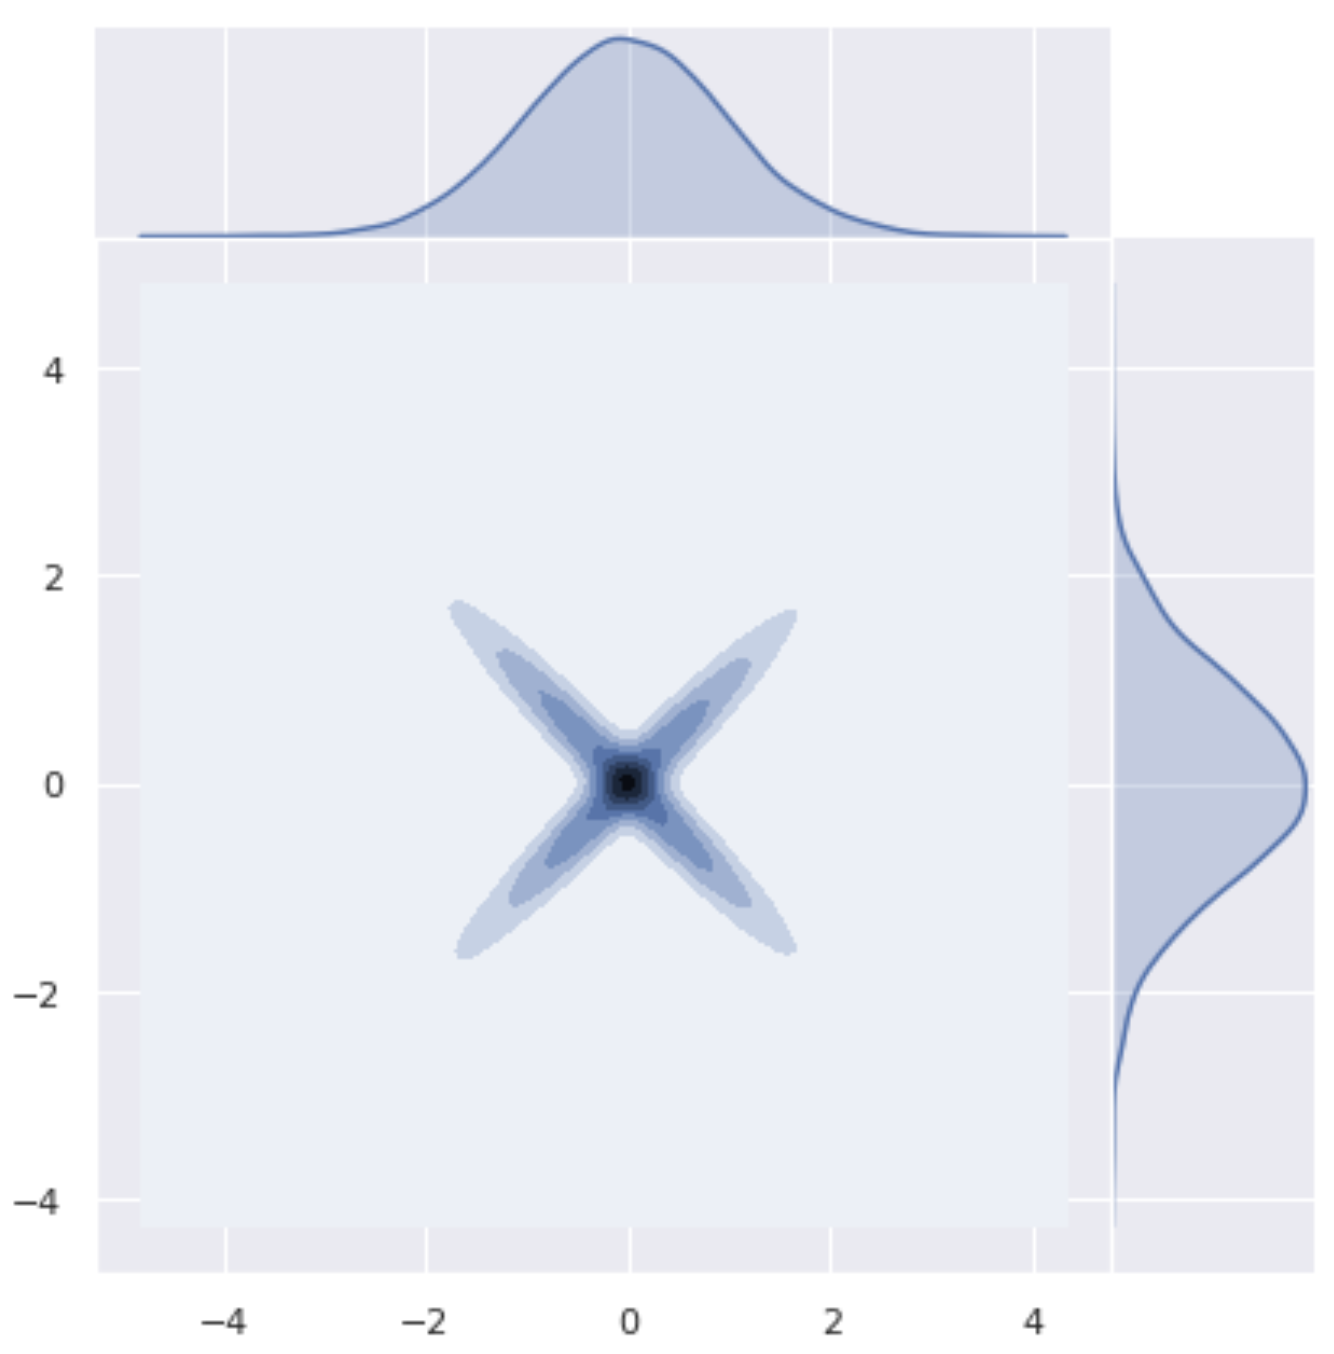
\includegraphics[scale=0.15]{images/no_multinormal_density.png} 
\caption{Left: Multivariate Normal Distribution, Right: Non-Multivariate Normal Distribution}
\end{figure}
\end{center}
\end{frame}


\section{Bayesian Linear Regression}


\begin{frame}{Bayesian Linear Regression}{\cite{reg_bayesian_regression_2019}, \cite[Chapter 2.1]{RW05}}
Let $x_1, \cdots, x_n \in \mathbb{R}^d$ and $y_1, \cdots, y_n$ be a set of observations (data). We want to fit the linear model 
$$
f(x) = x^T b \quad \text{and} \quad y = f(x) + \varepsilon, \quad \text{with} \quad \varepsilon \sim N(0, \sigma_n^2)
$$
where $b \in \mathbb{R}^d$ denotes the parameter vector. Let $X \in M_{d \times n}$ be denote the observation matrix. 
\begin{center}
\begin{figure}
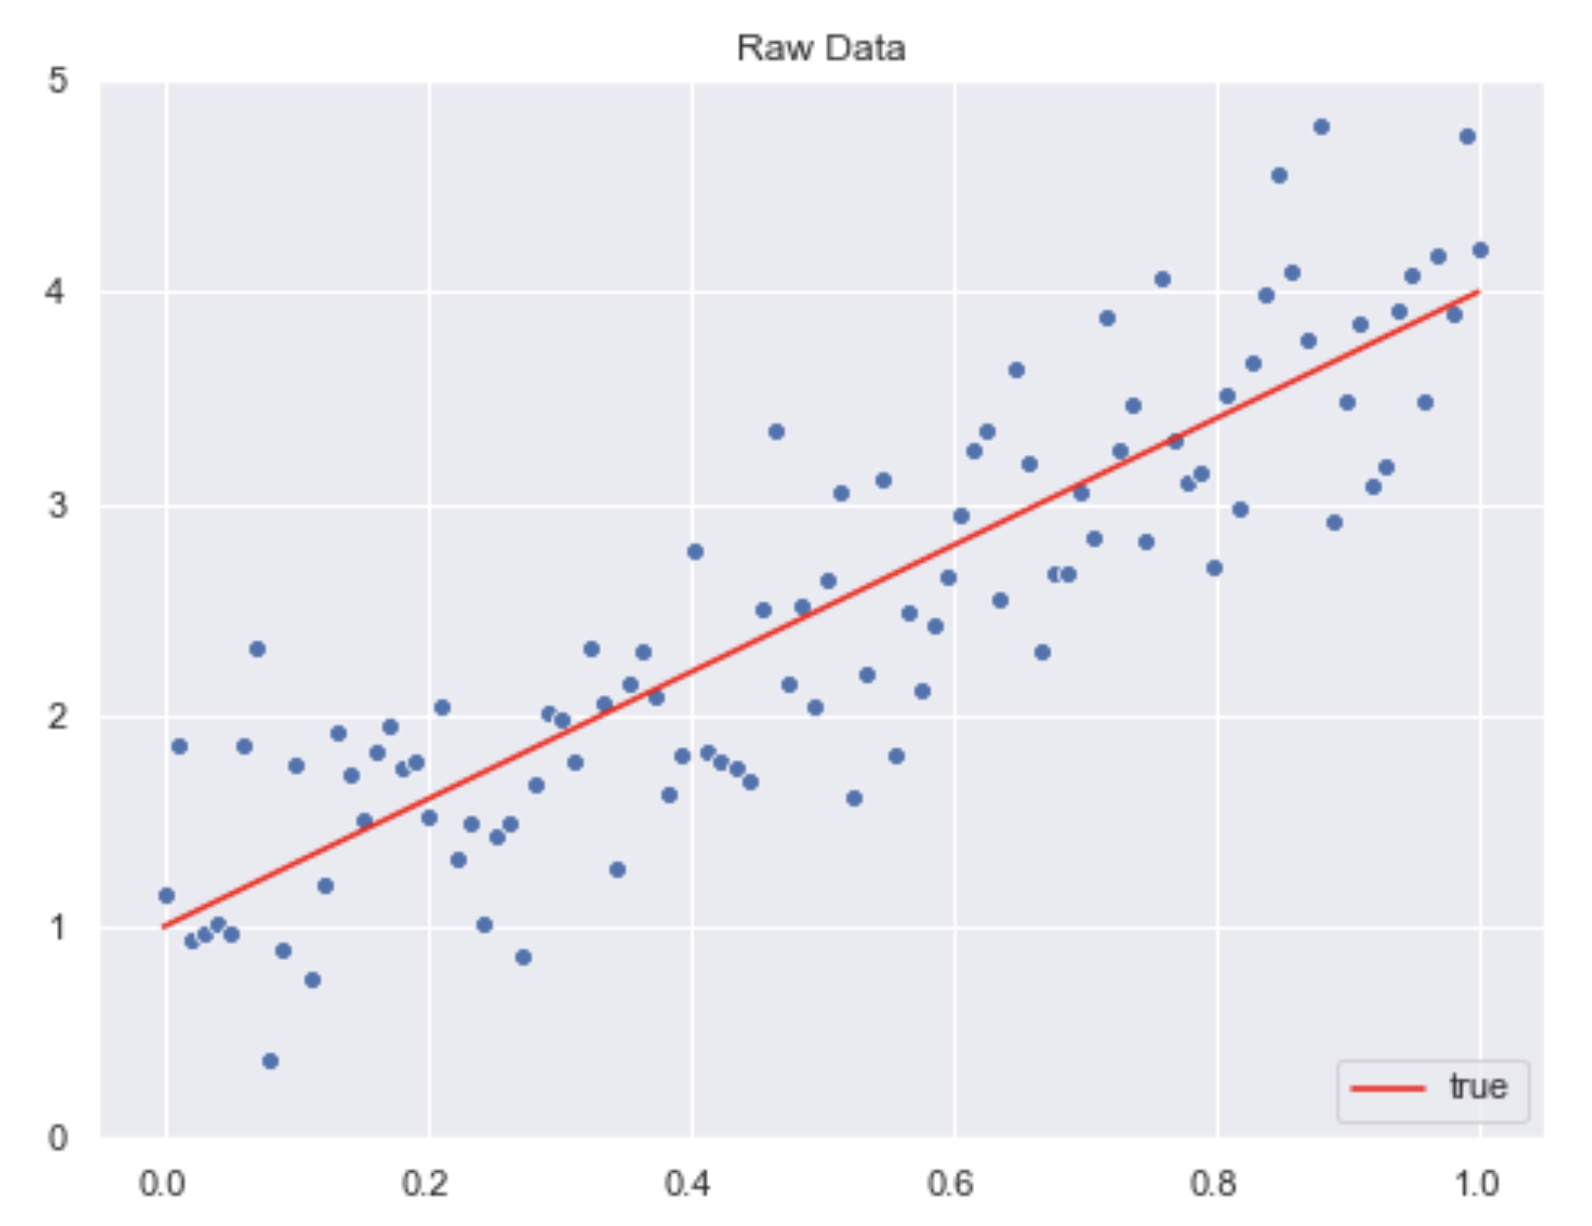
\includegraphics[scale=0.14]{images/lin_raw_data.png} 
\caption{The true parameters in this example are $b=(1, 3)$ and $\sigma_n=0.5$}
\end{figure}
\end{center}
We want to compute $p(b|X, y)$ using the Bayes theorem 
$$
p(b|X, y) = \frac{p(y|X, b) p(b)}{p(y|X) } \propto \text{likelihood} \times \text{prior}
$$
\end{frame}


\begin{frame}{Prior Distribution}
\begin{itemize}
\item Prior 
$$
b \sim N(0, \Sigma_p), \quad  \Sigma_p \in M_{d}(\mathbb{R})
$$

\begin{center}
\begin{figure}
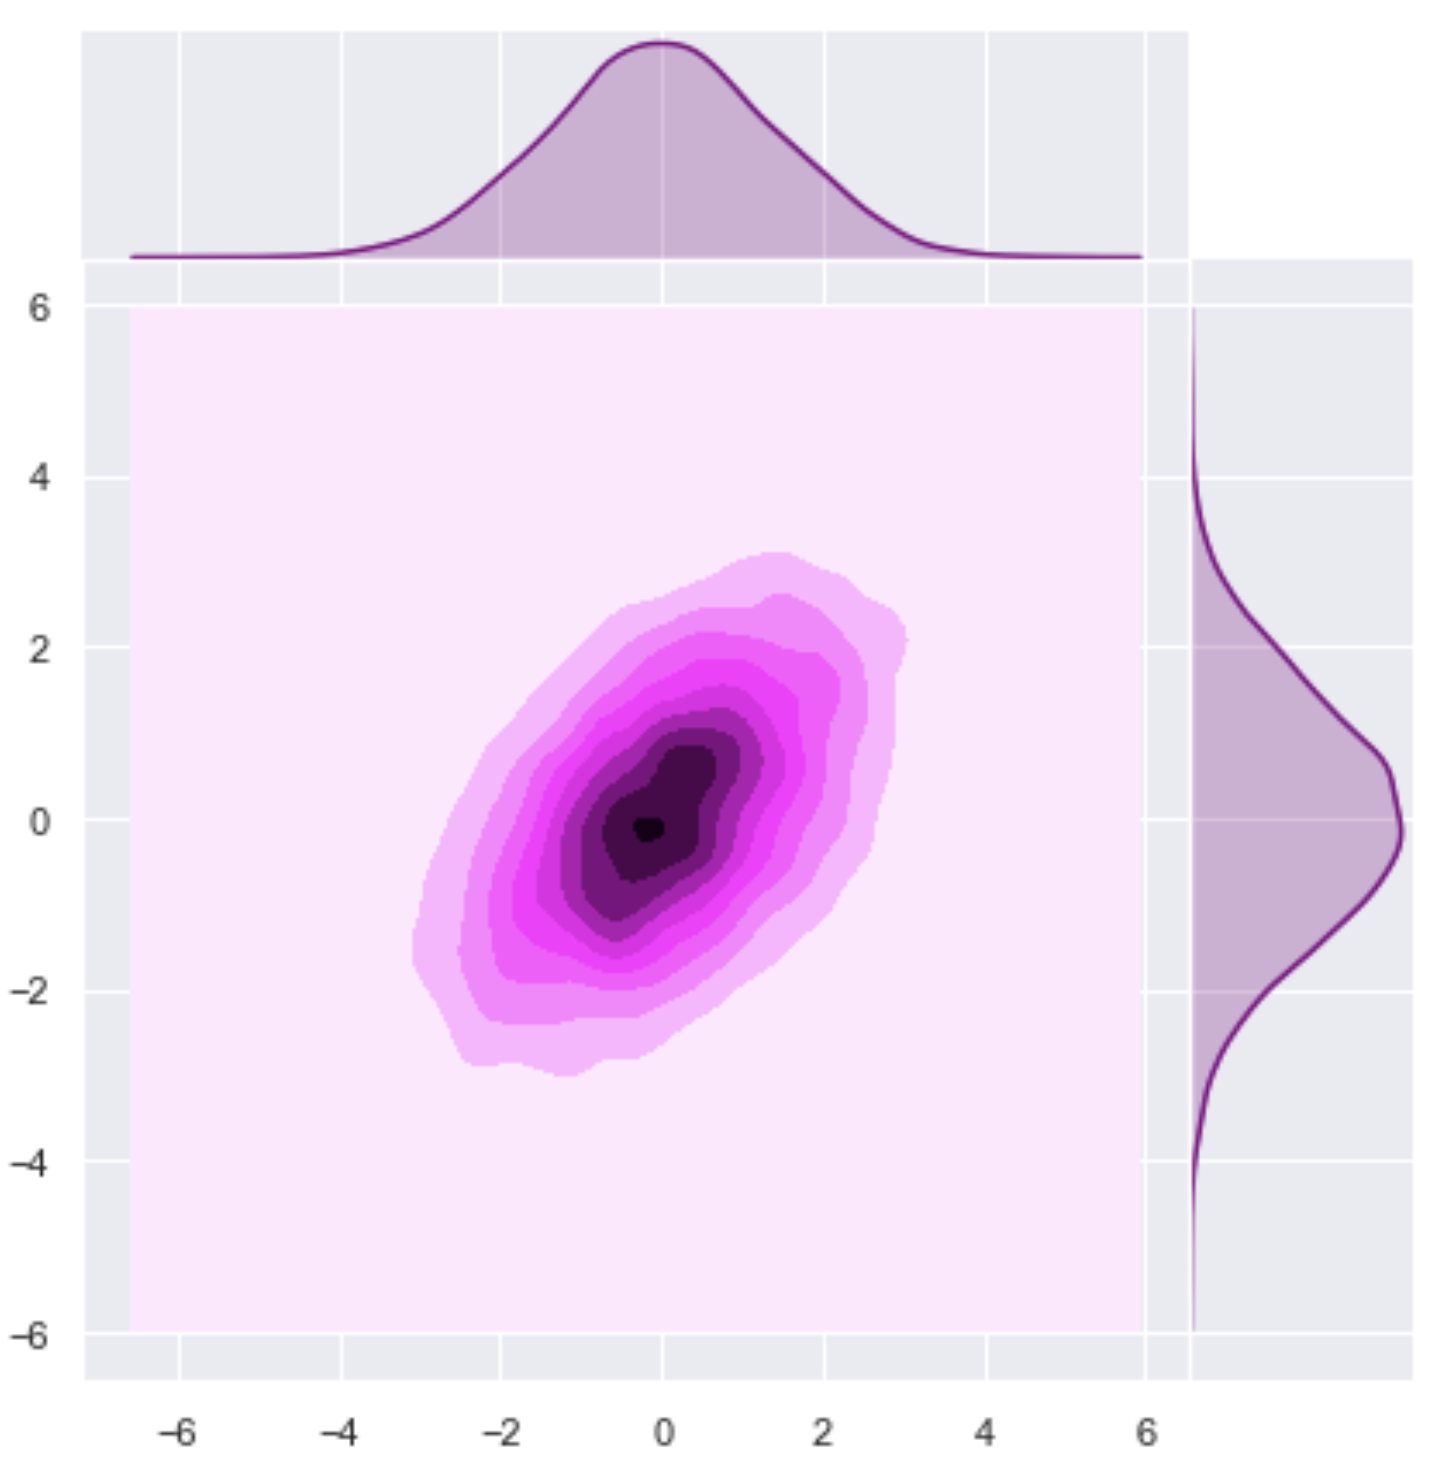
\includegraphics[scale=0.17]{images/lin_join_prior.png} 
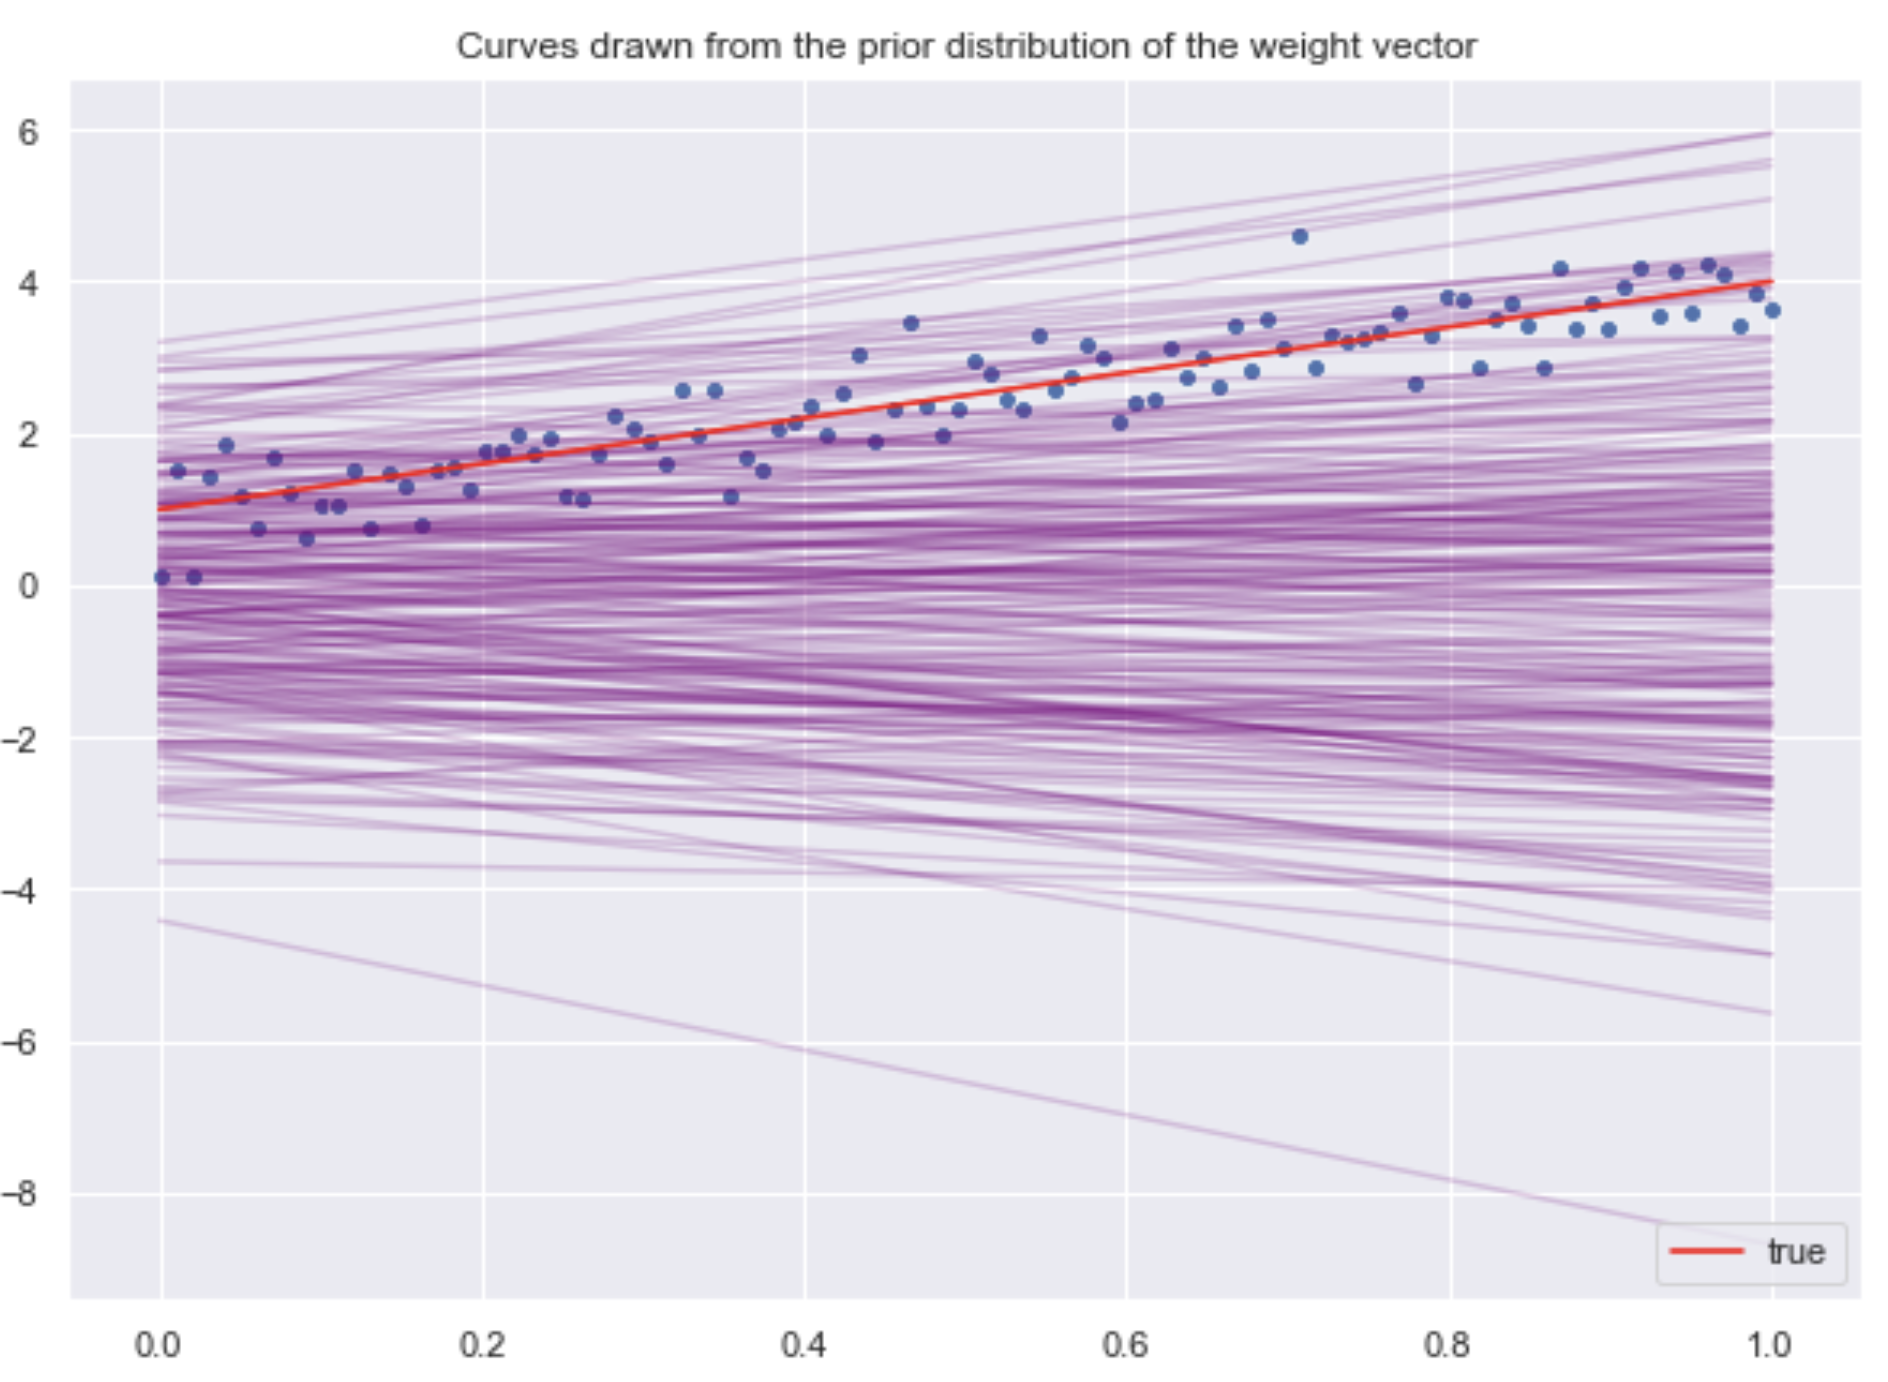
\includegraphics[scale=0.17]{images/prior_lin_mod_param_distr.png} 
\caption{Prior Distribution, for this example
$
\Sigma_p=
\left(
\begin{array}{cc}
2 & 1 \\
1 & 2
\end{array}
\right).
$
}
\end{figure}
\end{center}
\item Likelihood
\begin{align*}
p(y|X, b) 
= \prod_{i=1}^{n}p(y_i|x_i, b) 
%=& \frac{1}{(2\pi \sigma_n^2)^{n/2}} \exp\left(-\frac{1}{2\sigma_n^2}||y - X^T b||^2\right) \\
= N(X^T b, \sigma_n^2 I)
\end{align*}
\end{itemize}
\end{frame}

\begin{frame}{Posterior Distribution Sampling }{\cite{pymc3}}
\begin{center}
\begin{figure}
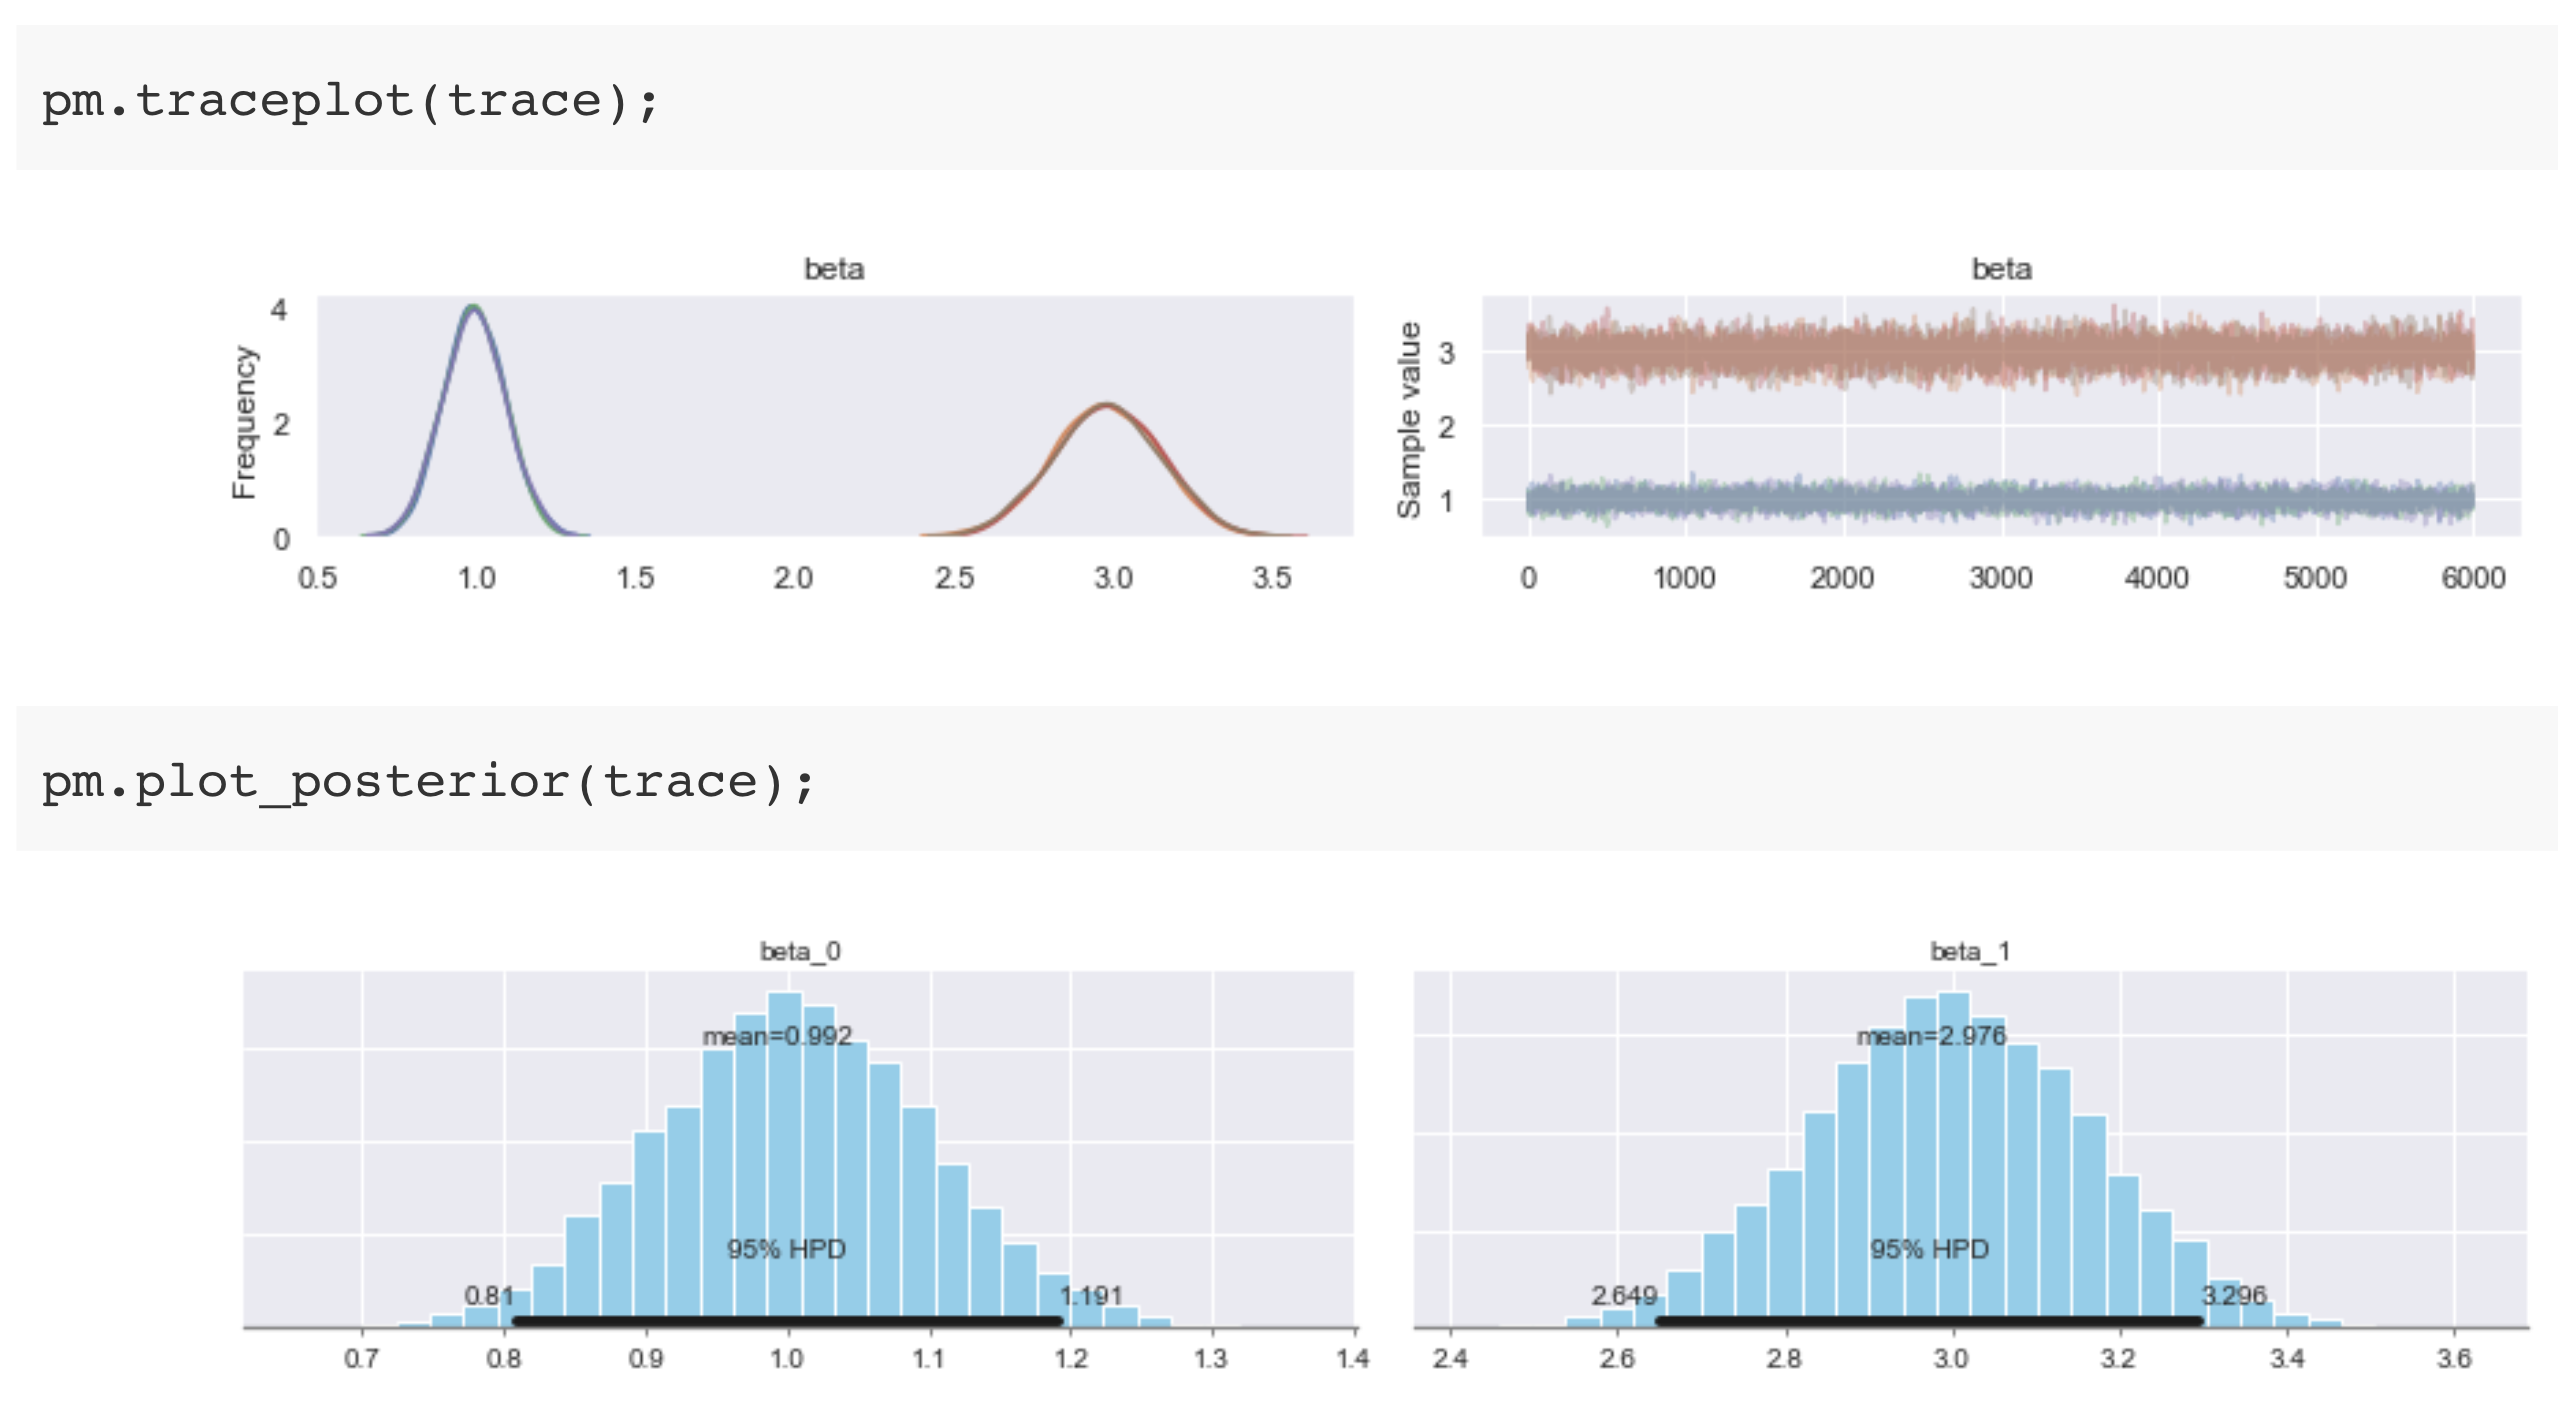
\includegraphics[scale=0.25]{images/lin_posterior_pymc3.png} 
\caption{Posterior distribution of the $b$ weight estimation using MCMC sampling (\href{https://docs.pymc.io/}{PyMC3}). Here we use 3 chains. }
\end{figure}
\end{center}
\end{frame}


\begin{frame}{Posterior Distribution - Analytical Solution}{\cite[Chapter 2.1.1]{RW05}}
\begin{itemize}
\item Posterior 
$$
p(b|y, X) = N\left(\bar{b}=\frac{1}{\sigma_n^2}A^{-1}Xy, A^{-1}\right), \quad A=\sigma_{n}^{-2}XX^T + \Sigma_p^{-1}
$$
\end{itemize}
\begin{center}
\begin{figure}
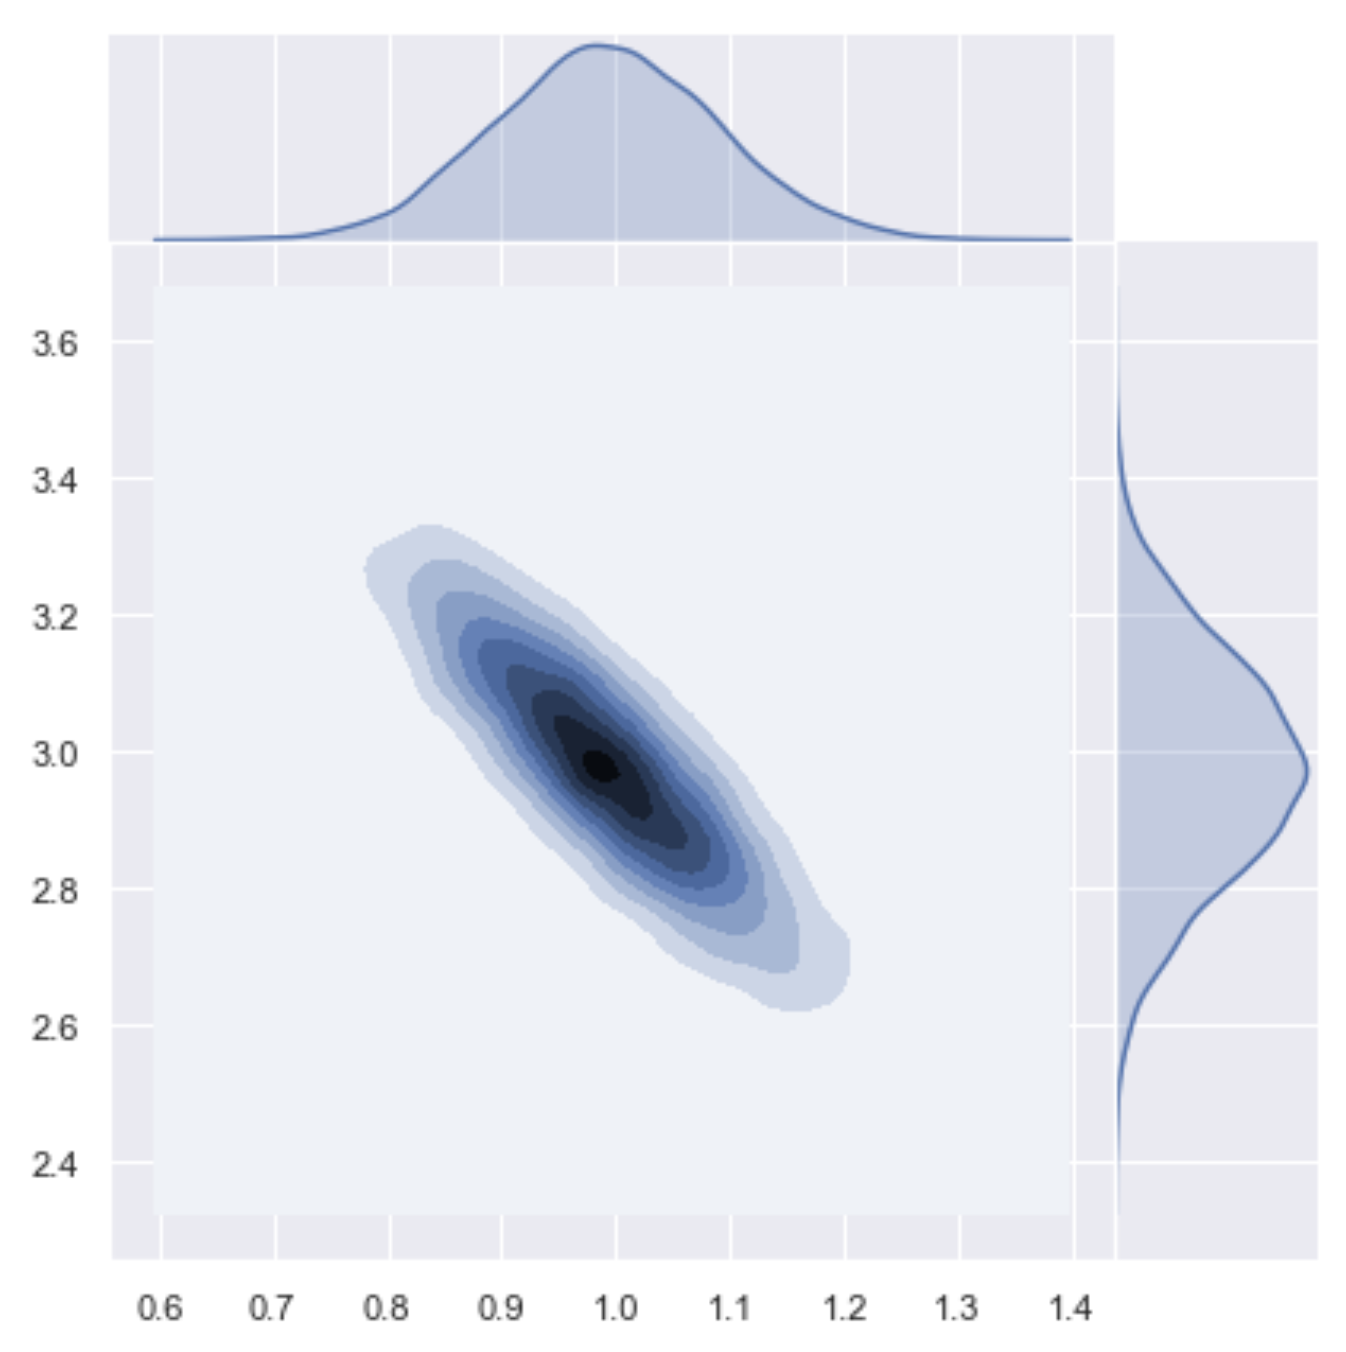
\includegraphics[scale=0.17]{images/lin_join_posterior.png} 
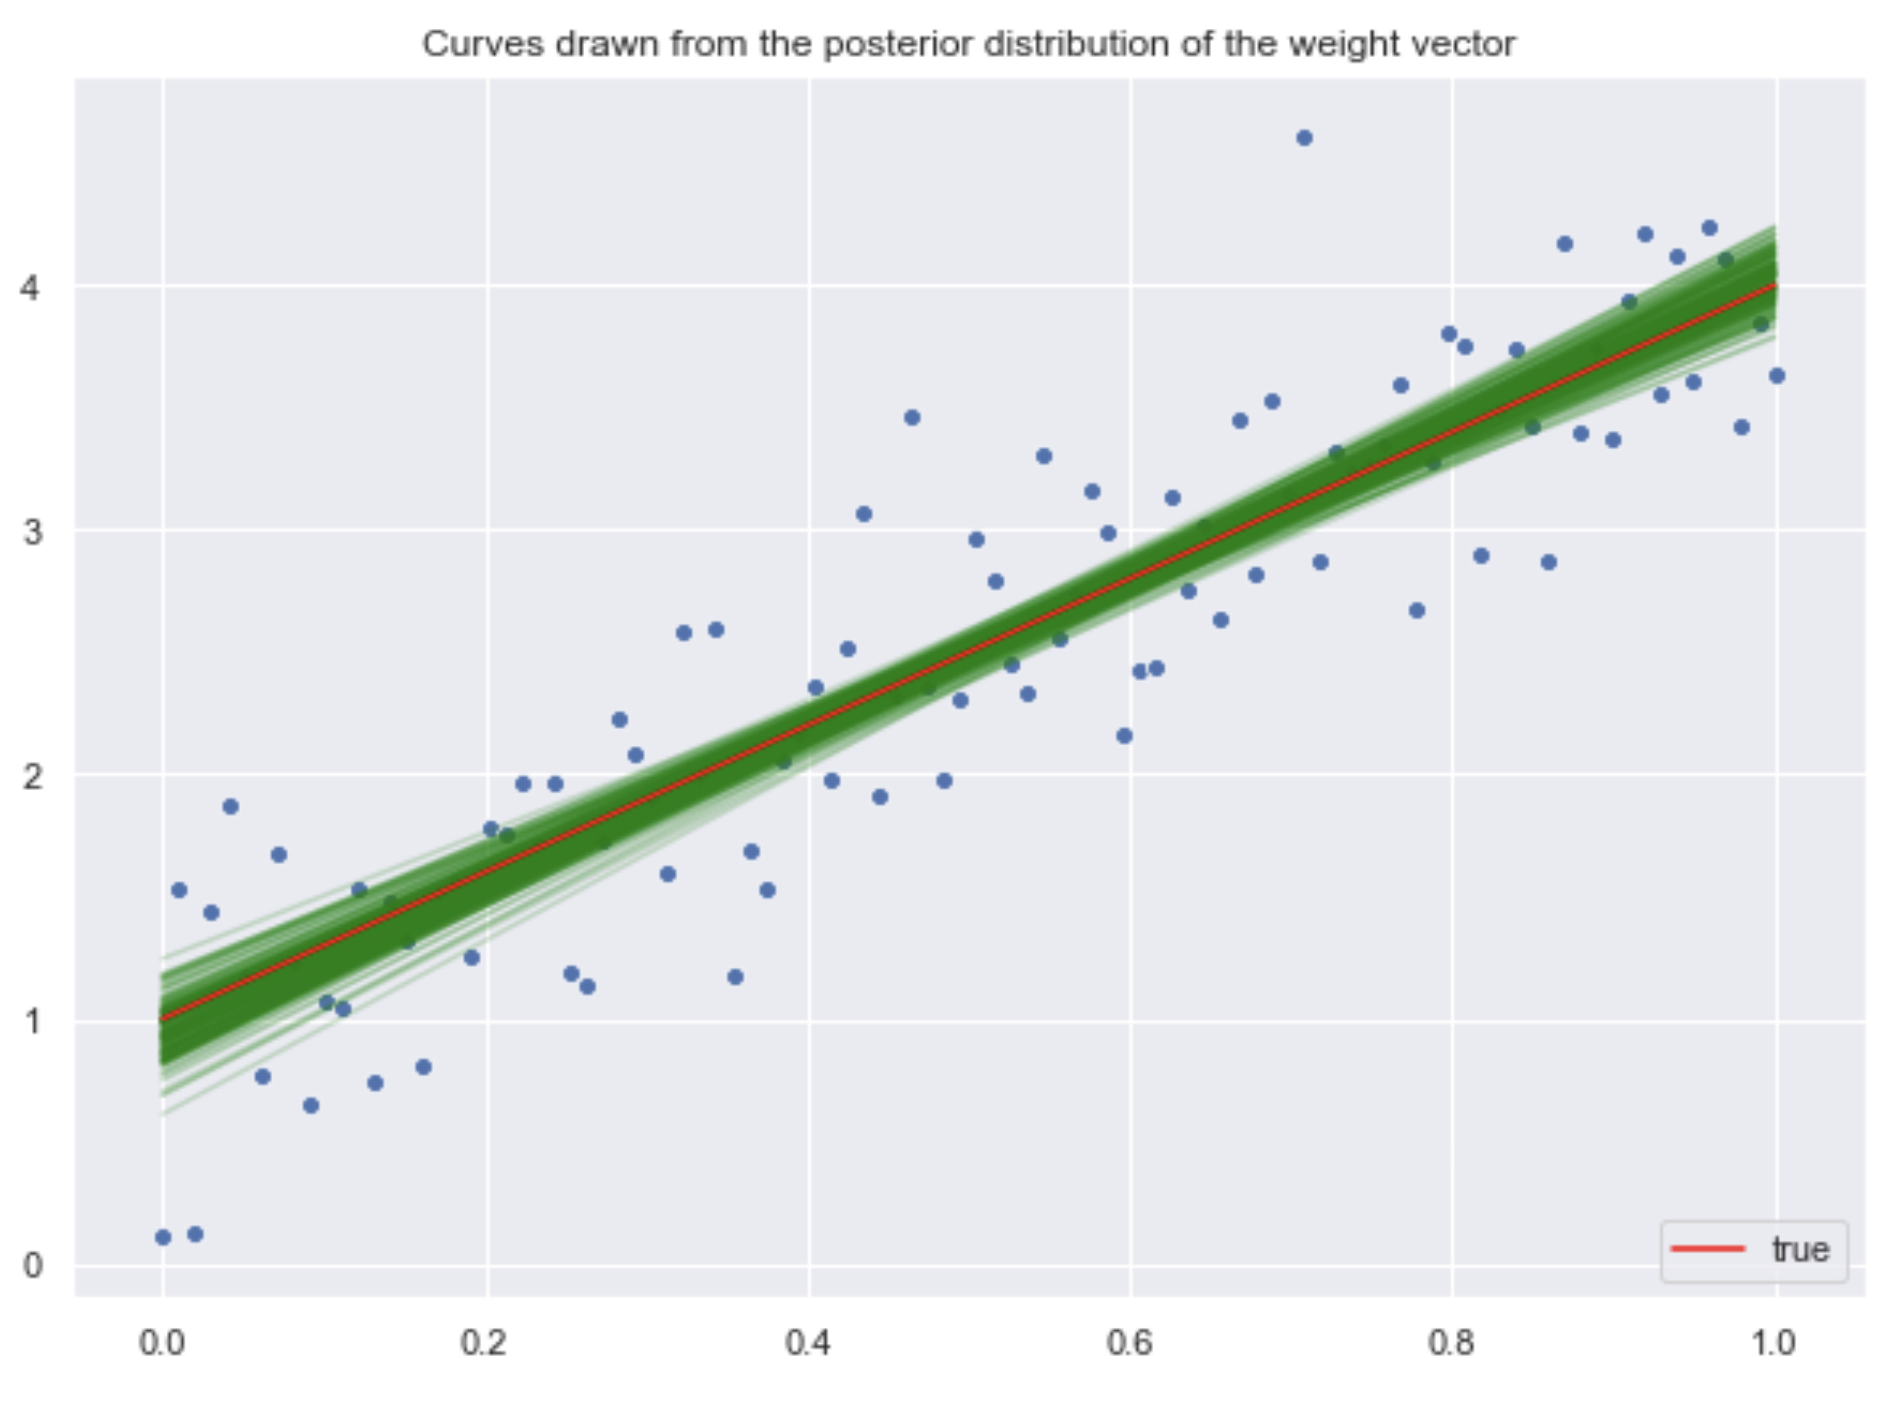
\includegraphics[scale=0.17]{images/posterior_lin_mod_param_distr.png} 
\caption{Posterior Distribution.}
\end{figure}
\end{center}
\end{frame}


\begin{frame}{Predictive Distribution - Analytical Solution}{\cite[Chapter 2.1.1]{RW05}}
\begin{align*}
p(f_*|x_*, X, y) 
= \int p(f_*|x_*, b)p(b|X, y)db 
= N\left(
\frac{1}{\sigma_n^2}x_*^T A^{-1}Xy, x_*^T A^{-1}x_*
\right)
\end{align*}

\begin{center}
\begin{figure}
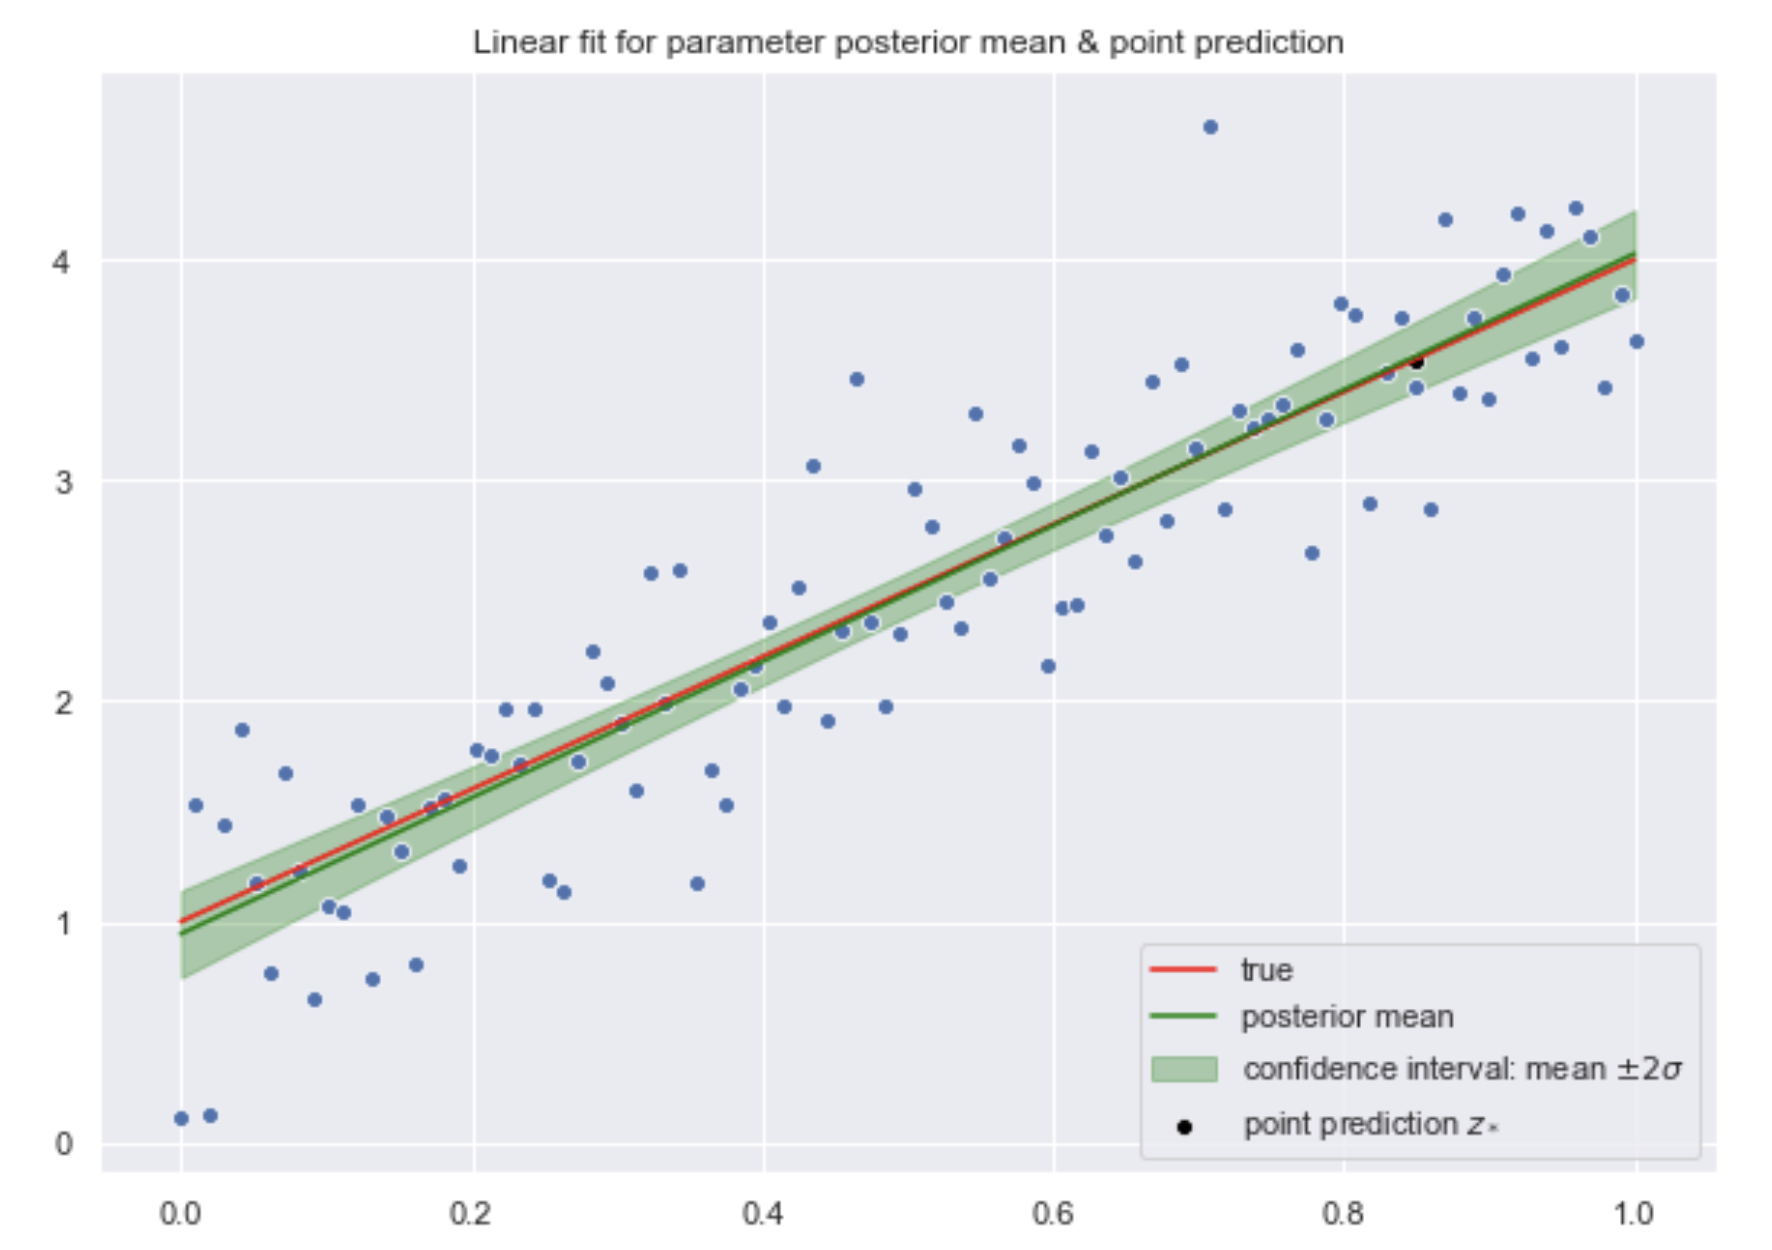
\includegraphics[scale=0.25]{images/lin_prediction.png} 
\caption{Prediction Interval.}
\end{figure}
\end{center}
\end{frame}


\section{The Kernel Trick}


\begin{frame}{The Kernel Trick}{\cite[Chapter 2.1.2]{RW05}}
Let us consider a map $\phi: \mathbb{R}^d \longrightarrow \mathbb{R}^N$ and the model
$$
f(x) = \phi(x)^T b \quad \text{and} \quad y = f(x) + \varepsilon, \quad \text{with} \quad \varepsilon \sim N(0, \sigma_n^2). 
$$
It is easy to verify that the analysis for this model as analogous to the standard linear model replacing $X$ with $\Phi\coloneqq \phi(X)$. Set $\phi_*= \phi(x_*)$, 
\begin{align*}
p(f_*|x_*, X, y) =& N\left(
\overbrace{\frac{1}{\sigma_n^2}\phi_*^T A^{-1}\Phi y}^{(1)},
\underbrace{ \phi_*^T A^{-1}\phi_*}_{(2)}
\right)
\end{align*}
\begin{align*}
(1) =& \phi_{*}^T \Sigma_{p}\Phi(\Phi^T \Sigma_p \Phi + \sigma_n^2I)^{-1}y \\
(2)= &\phi_{*}^T\Sigma_p\phi_{*} - \phi_{*}^T \Sigma_{p}\Phi(\Phi^T \Sigma_p \Phi + \sigma_n^2I)^{-1}\Phi^T\Sigma_p\phi_*
\end{align*}
This motivates the definition of the {\bf covariance function} or {\bf kernel}
$$
k(x, x')\coloneqq \phi(x)^T\Sigma_p\phi(x')
$$
\end{frame}


\section{Gaussian Process Regression}


\begin{frame}{Gaussian Process}{\cite[Chapter 21]{BDA13}, \cite[Chapter 2.2]{RW05}}
\begin{block}{Main Idea}
The specification of a covariance function implies a distribution over functions.
\end{block}
\begin{block}{Gaussian Process}
\begin{itemize}
\item A {\bf Gaussian Process} is a collection of random variables, any finite number of which have a joint multinormal distribution. \\
\item A Gaussian process $f \sim \mathcal{GP}(m, k)$ is completely specified by its mean function $m(x)$ and covariance function $k(x, x')$. Here $x \in \mathcal{X}$ denotes a point on the index set $\mathcal{X}$.
$$
m(x) = E[f(x)]
\quad
\text{and}
\quad
k(x, x') = E[(f(x) - m(x))(f(x') - m(x'))]
$$
\end{itemize}
\end{block}
\pause 
\begin{block}{Example}
The map $f(x) = \phi(x)^T b $ (with prior $b\sim N(0, \Sigma_p)$) defines a Gaussian process with $m(x)=0$ and $k(x, x') = \phi(x)^T\Sigma_p\phi(x')$.
\end{block}
\begin{block}{Notation}
Let $K(X, X)$ denote the matrix of the point-wise kernel images. 
\end{block}
\end{frame}

\begin{frame}{Linear Regression - Function Space View}{\cite[Chapter 2.2]{RW05}}
\begin{itemize}
\item Let us consider input points $X_*$ (test set).
\item Prior
\begin{align*}
f_* \sim N(0, K(X_*,X_* ))
\end{align*}
\begin{center}
\begin{figure}
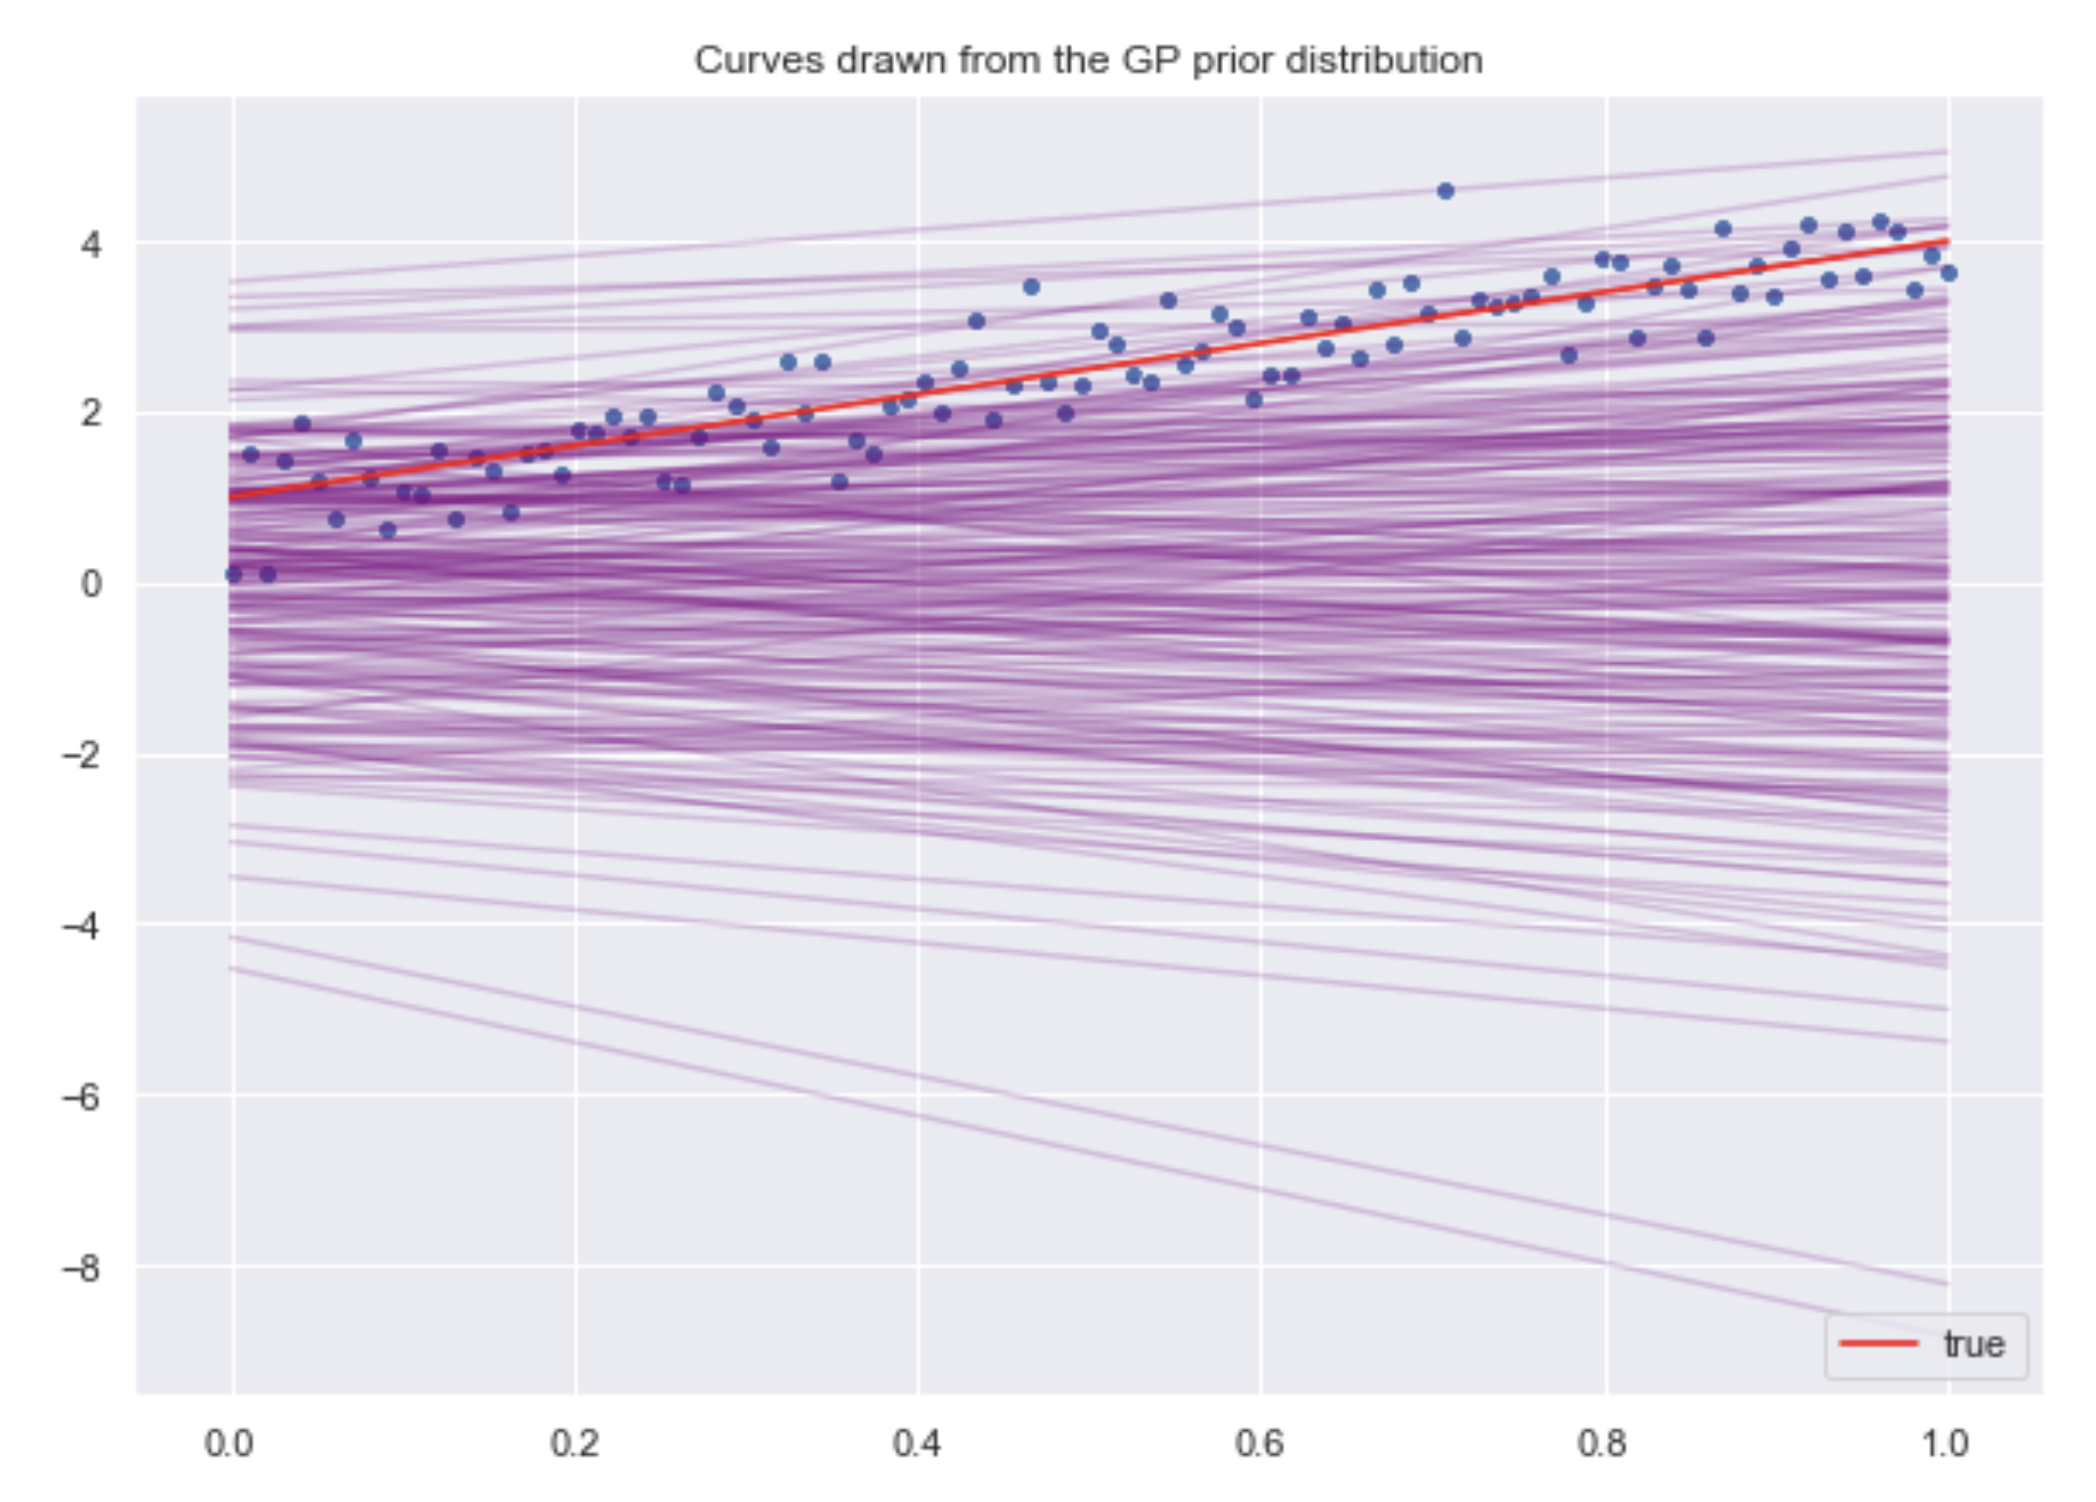
\includegraphics[scale=0.2]{images/gp_lin_prior.png} 
\caption{We sample from the prior space of functions by plotting their realization on $n_*=80$ points. }
\end{figure}
\end{center}
\end{itemize}
\end{frame}


\begin{frame}{Linear Regression - Function Space View}{\cite[Chapter 2.2]{RW05}}
\begin{itemize}
\item Joint Distribution
\begin{align*}
\left(
\begin{array}{c}
y \\
f_*
\end{array}
\right)
\sim
N\left(0, 
\left(
\begin{array}{cc}
K(X,X)+\sigma_n^2 & K(X,X_*) \\
K(X_*,X) & K(X_*,X_*)
\end{array}
\right)
\right)
\end{align*}
\item Conditional Distribution $f_* | X, y, X_*\sim N(\bar{f}_*, \text{cov}(f_*))$
\begin{center}
\begin{figure}
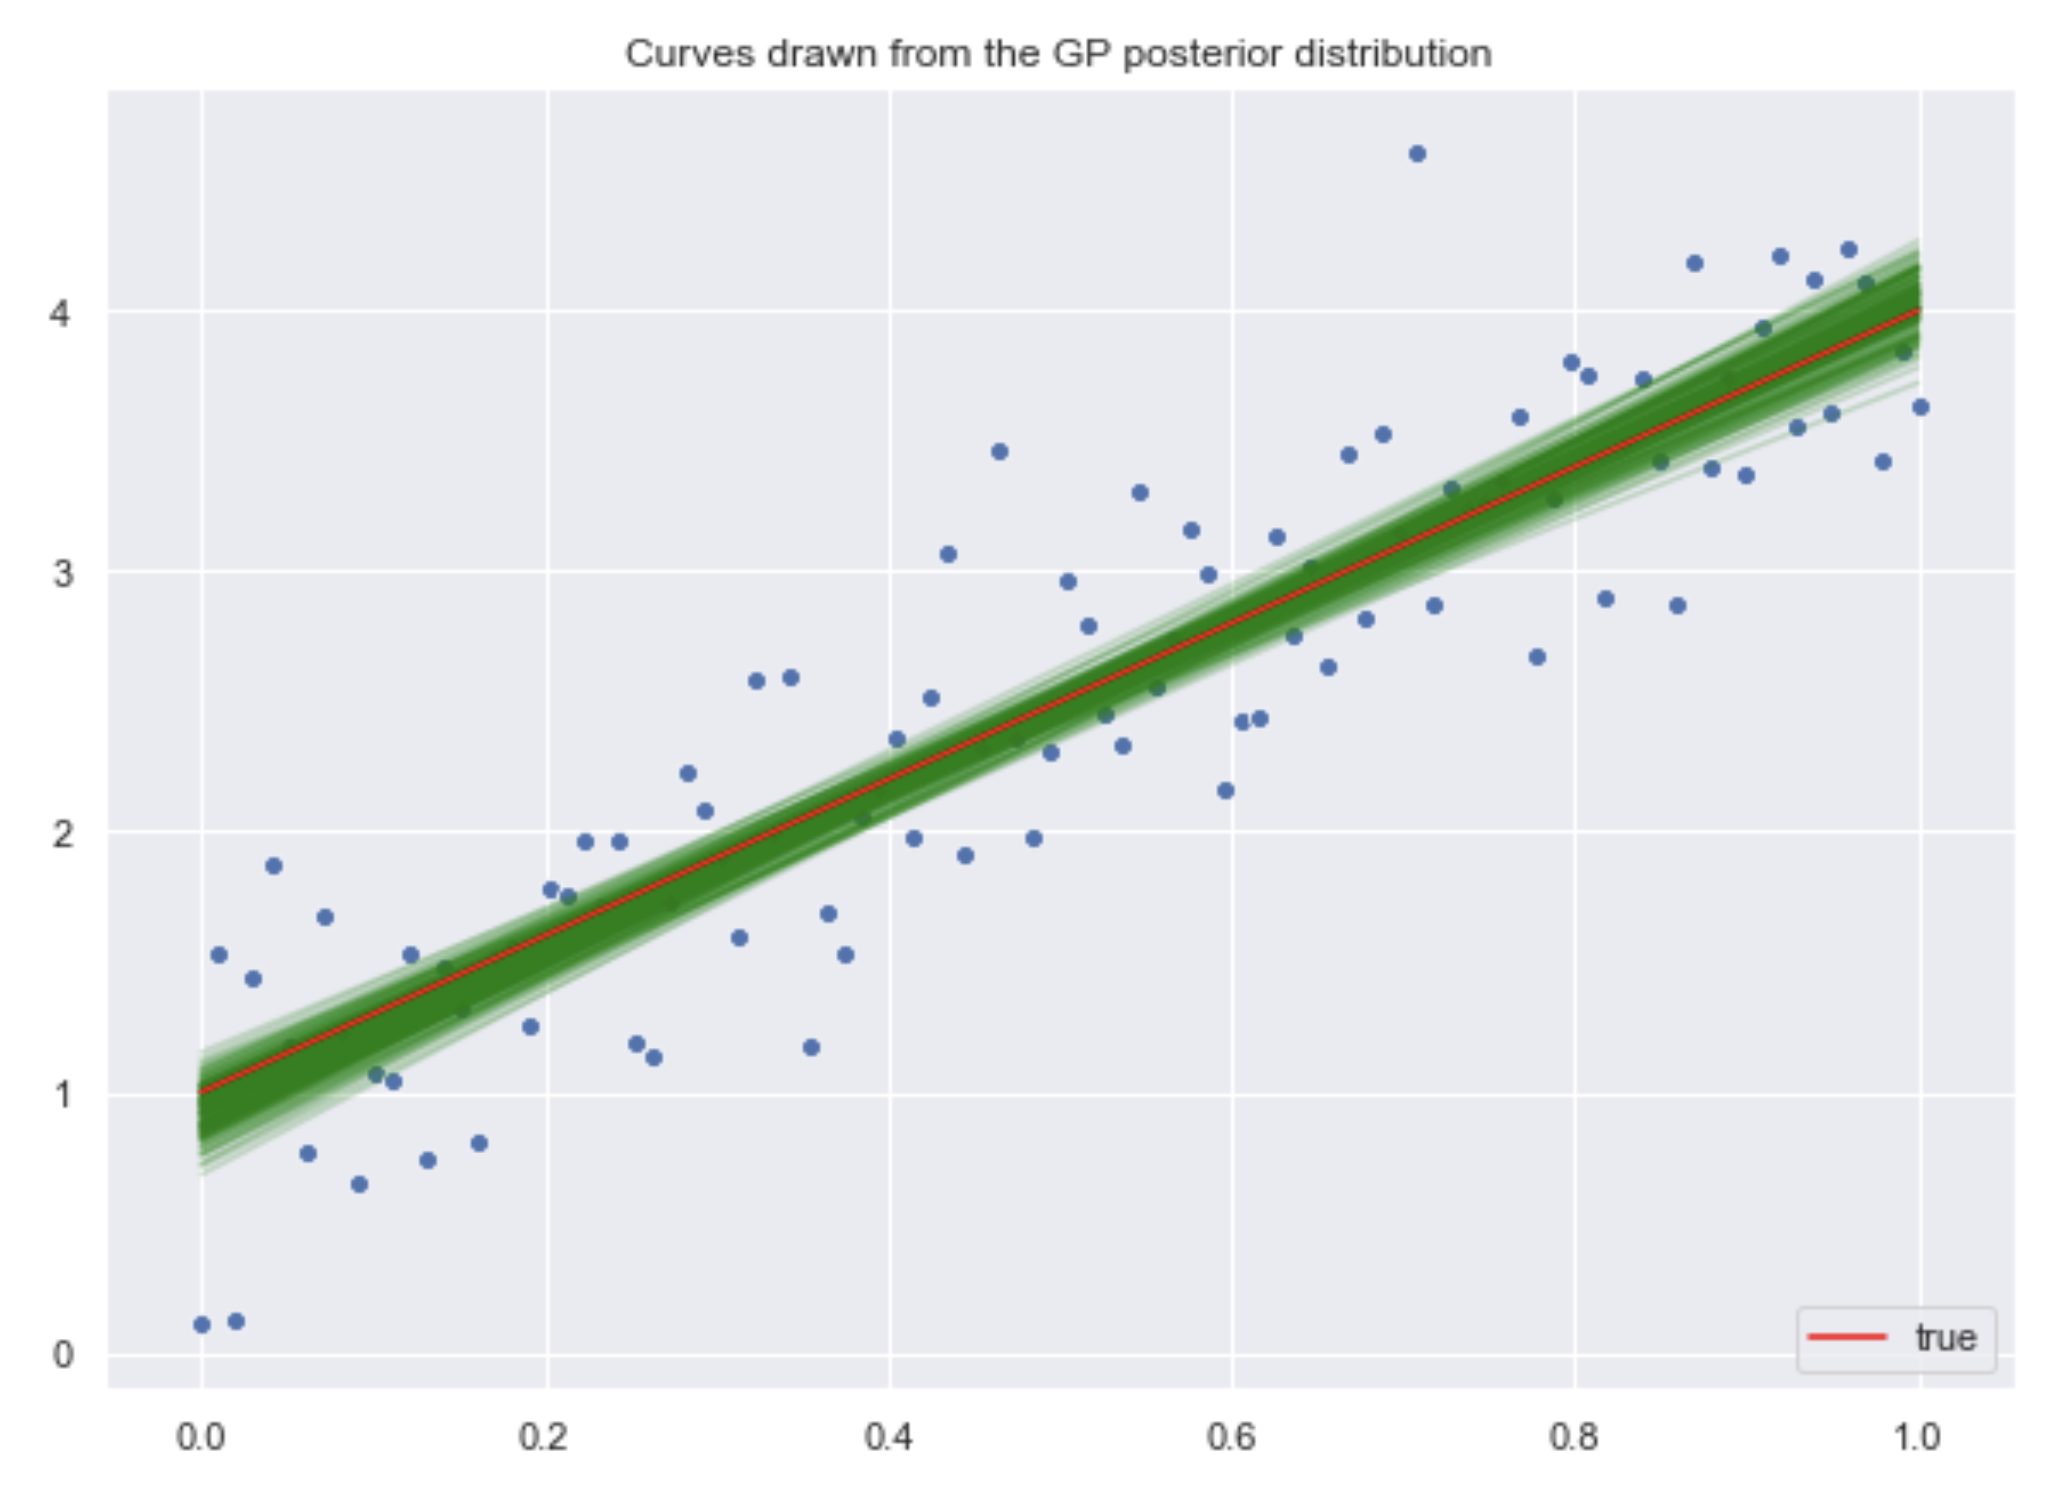
\includegraphics[scale=0.15]{images/gp_lin_posterior.png} 
\end{figure}
\end{center}
\begin{align*}
\bar{f}_* =& K(X_*,X)(K(X,X) + \sigma_n^2 I)y \\
 \text{cov}(f_*) =& K(X_*,X_*) - K(X_*,X)(K(X,X) + \sigma_n^2I)^{-1}K(X,X_*)
\end{align*}
\end{itemize}
\end{frame}


\section{Kernel Examples}


\begin{frame}{Kernel Examples}{\cite{ROERGA}, \cite[Chapter 4.2]{RW05}}
Symmetric and positive semi-definite functions $k:\mathcal{X}\times\mathcal{X}\longrightarrow \mathbb{R}$. 
\begin{itemize}
\item Dot Product 
\begin{align*}
k_{DOT}(x, x') = (\sigma_0^2 + x^T\Sigma_p x')^m
\end{align*}
\item Squared Exponential 
\begin{align*}
k_{SE}(x, x') = \exp\left(- \frac{(x - x')^2}{2\ell ^2}\right)
\end{align*}
\item Rational Quadratic 
\begin{align*}
k_{RQ}(x, x') = \left(1 + \frac{(x - x')^2}{2\alpha\ell^2}\right)^{-\alpha}
\end{align*}
\item Exp-Sine-Squared 
\begin{align*}
k_{ESS} (x, x')= \exp\left(-2 \left(\frac{\sin(\pi (x - x')/T )}{\ell}\right)^2\right)
\end{align*}
\end{itemize}
\end{frame}

\section{Non-Linear Example (RBF)}

\begin{frame}{Example: Non-Linear Function}{\cite{gaussian_process_reg_2019}}
\begin{center}
\begin{figure}
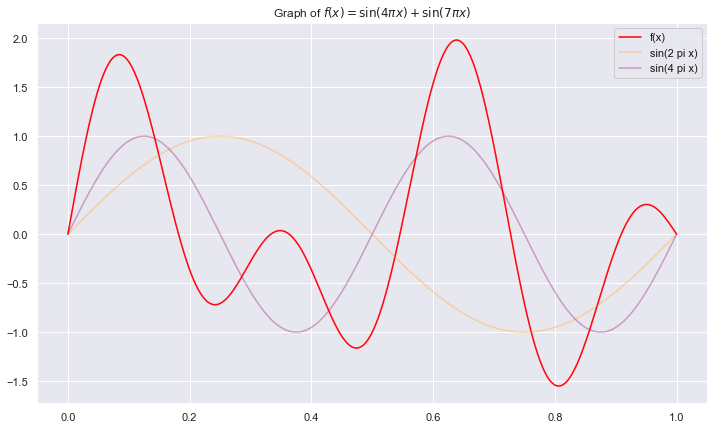
\includegraphics[scale=0.23]{images/f_example2.png} 
\end{figure}
\end{center}
\begin{center}
\begin{figure}
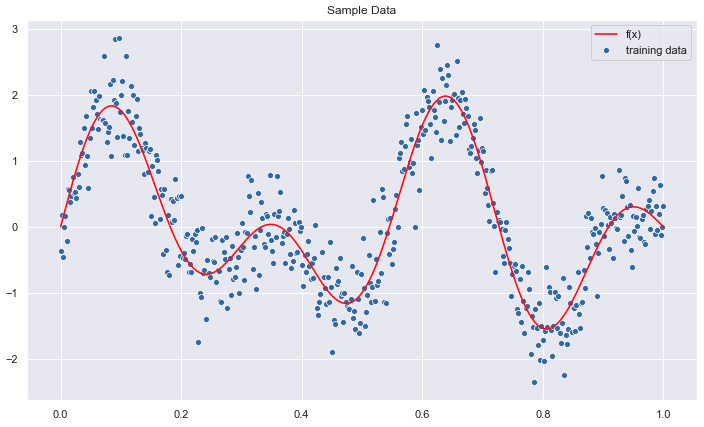
\includegraphics[scale=0.23]{images/raw_data_example2.png} 
\caption{Non-Linear Example with $n=500$ training points.}
\end{figure}
\end{center}
\end{frame}

\begin{frame}{Prior Distribution}
$$
f \sim N(0, K(X_*,X_*))
$$
\begin{center}
\begin{figure}
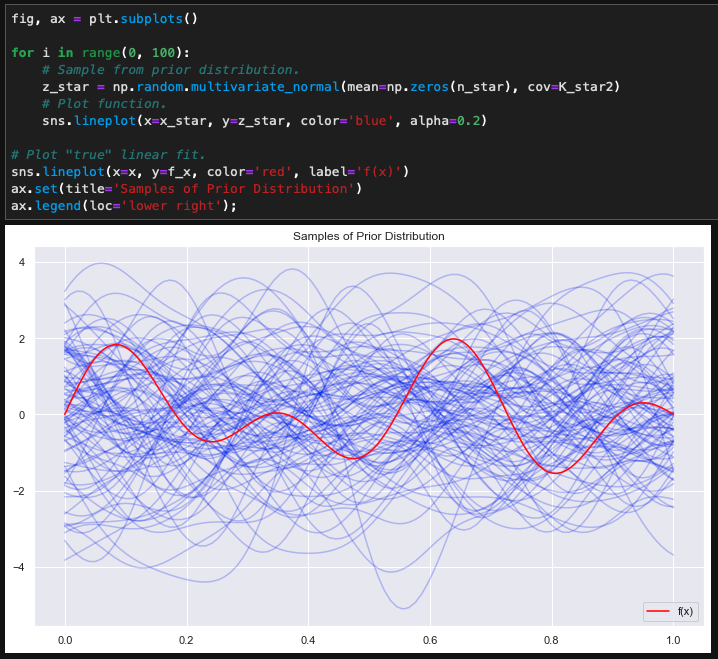
\includegraphics[scale=0.27]{images/code_sample_prior_example2.png} 
\caption{We sample from the prior space of functions by plotting their realization on $n_*=100$ points. }
\end{figure}
\end{center}
\end{frame}


\begin{frame}{Joint Distribution}
\begin{align*}
\left(
\begin{array}{c}
y \\
f_*
\end{array}
\right)
\sim
N\left(0, 
\left(
\begin{array}{cc}
K(X,X)+\sigma_n^2 & K(X,X_*) \\
K(X_*,X) & K(X_*,X_*)
\end{array}
\right)
\right)
\end{align*}
\begin{center}
\begin{figure}
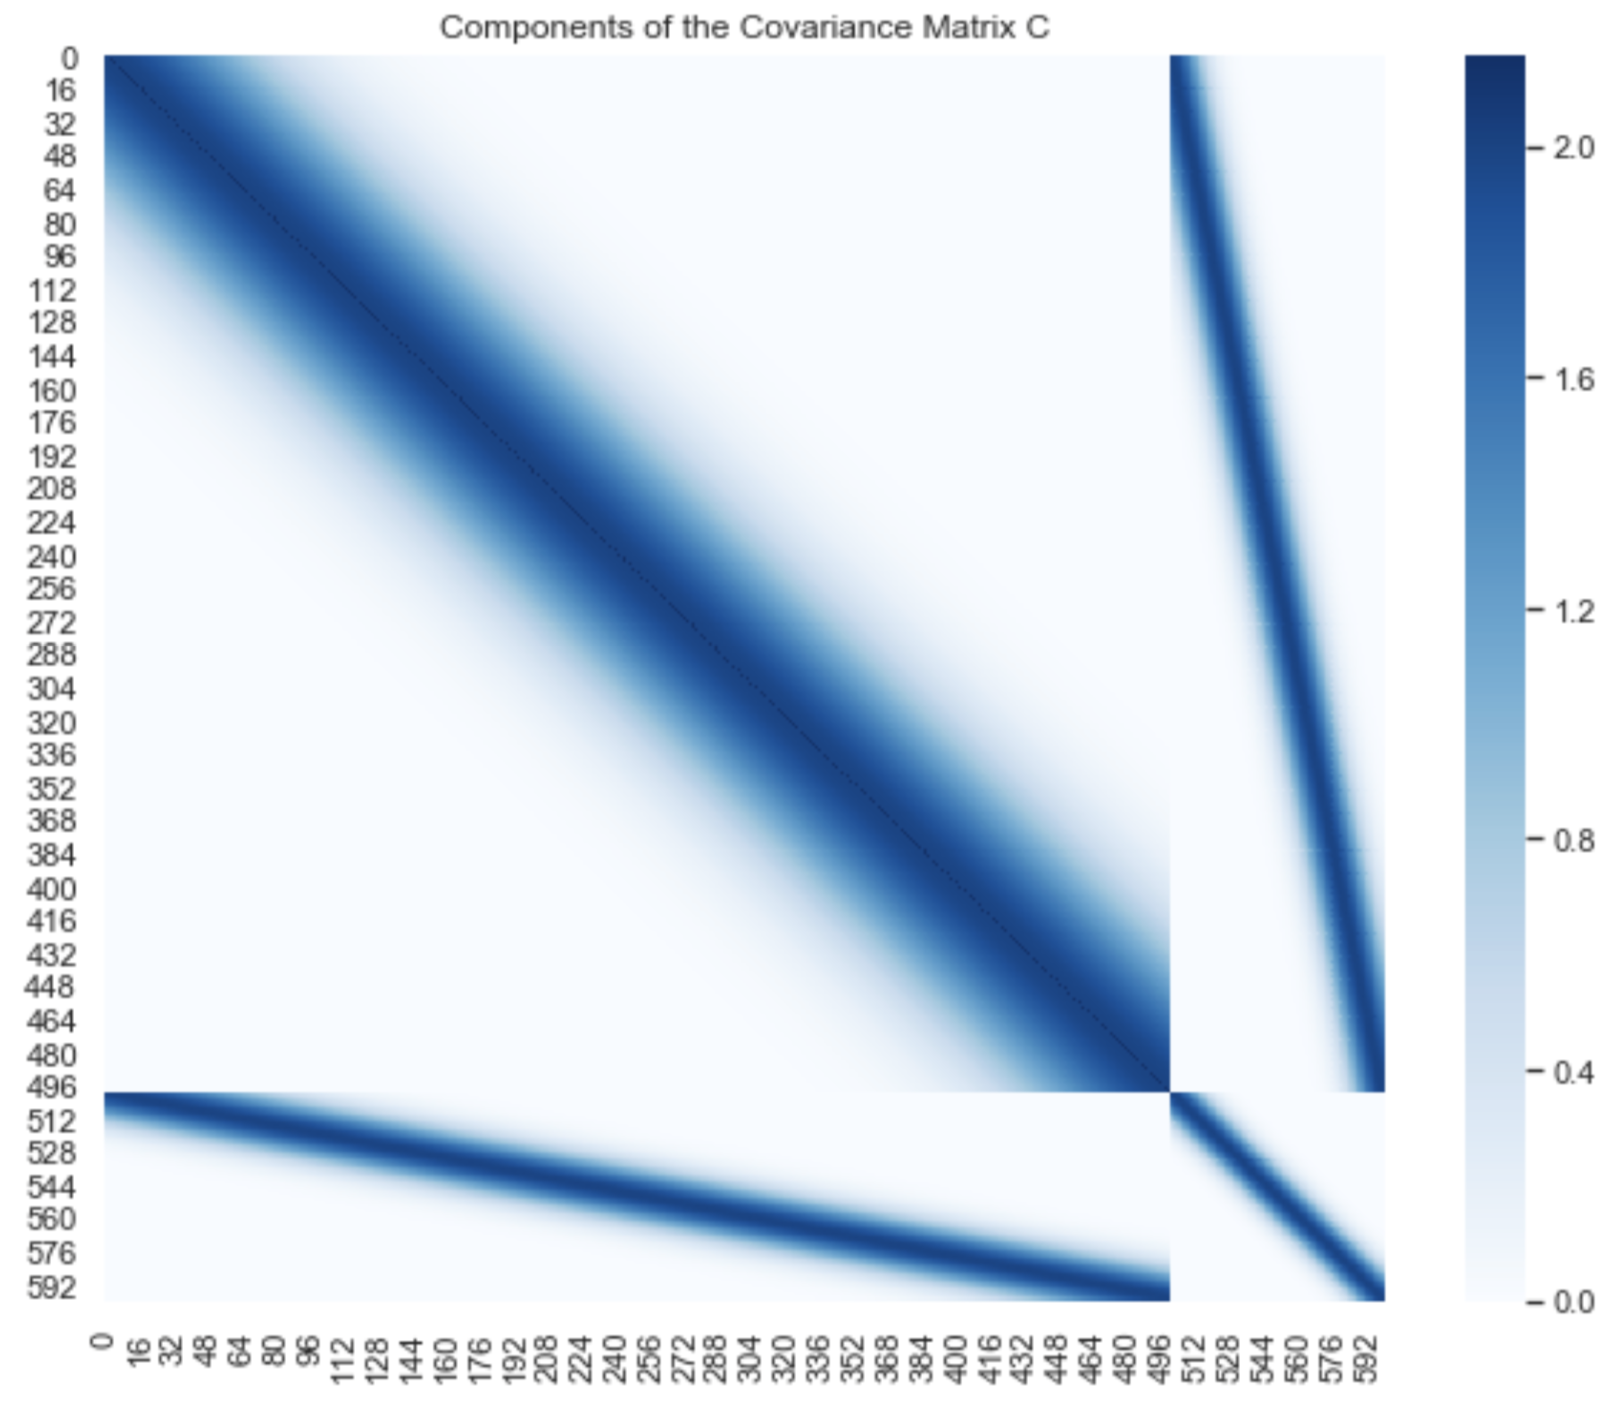
\includegraphics[scale=0.25]{images/cov_prior_example2.png} 
\end{figure}
\end{center}
\end{frame}


\begin{frame}{Conditional Distribution}
 $$f_* | X, y, X_*\sim N(\bar{f}_*, \text{cov}(f_*))$$
\begin{center}
\begin{figure}
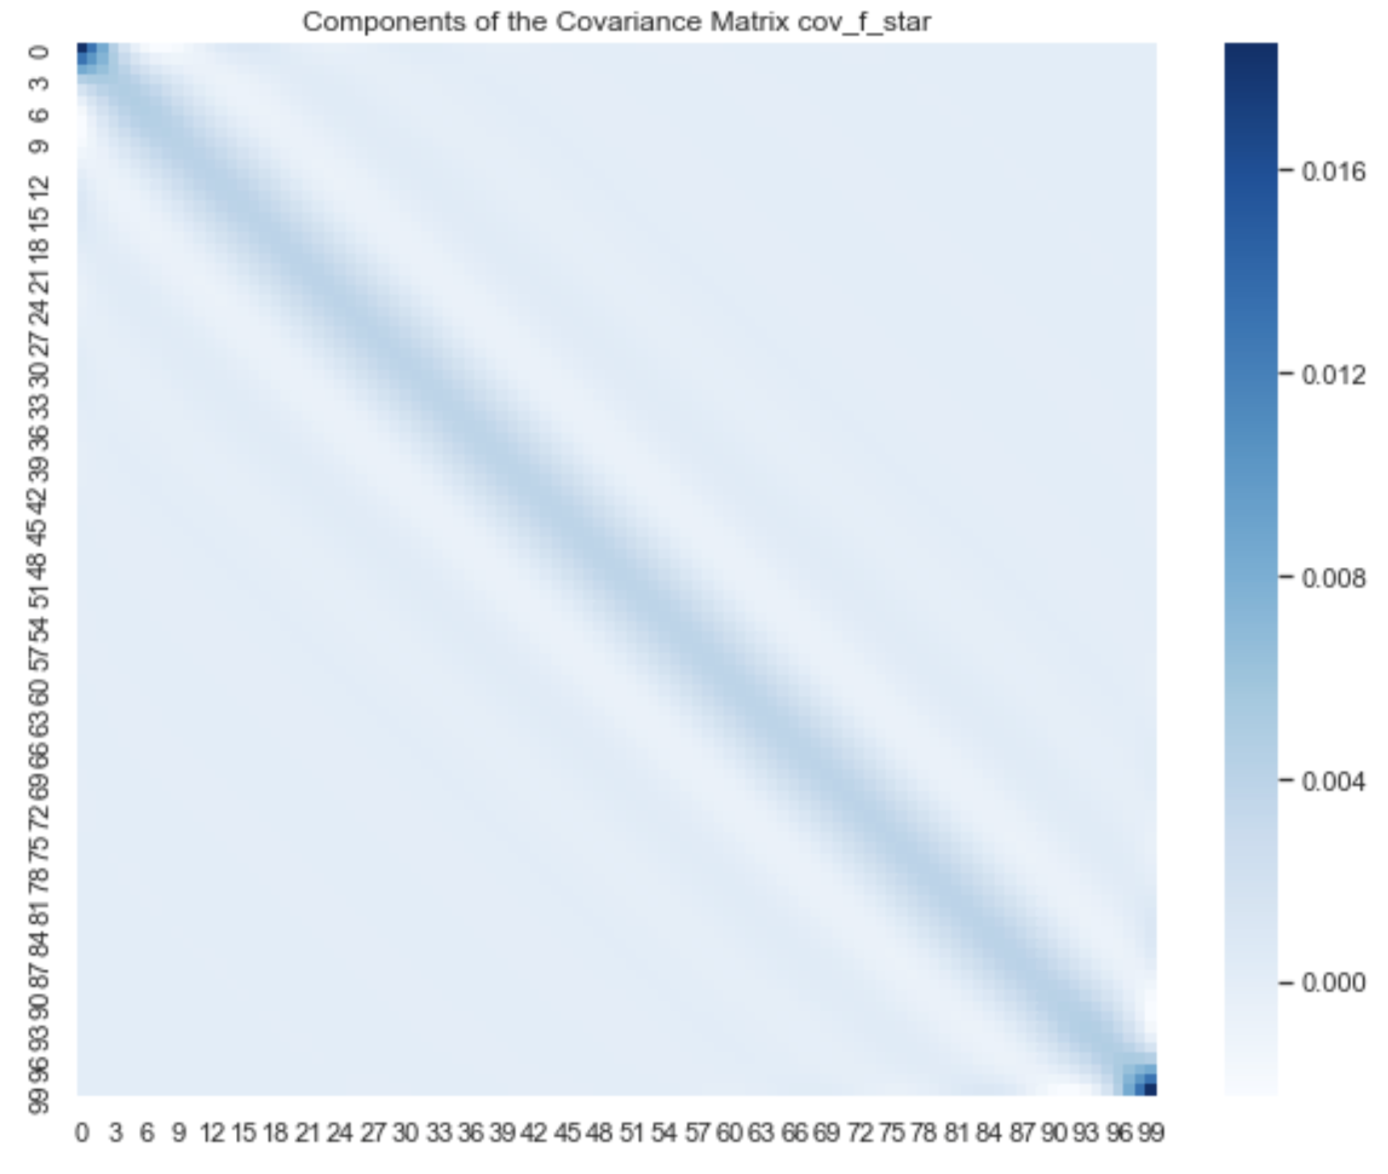
\includegraphics[scale=0.24]{images/cov_posterior_example2.png} 
\caption{Covariance matrix of the posterior (conditional) distribution.}
\end{figure}
\end{center}
 \begin{align*}
\bar{f}_* =& K(X_*,X)(K(X,X) + \sigma_n^2 I)y \\
\text{cov}(f_*) =& K(X_*,X_*) - K(X_*,X)(K(X,X) + \sigma_n^2I)^{-1}K(X,X_*)
\end{align*}
\end{frame}


\begin{frame}{Posterior Distribution}
\begin{center}
\begin{figure}
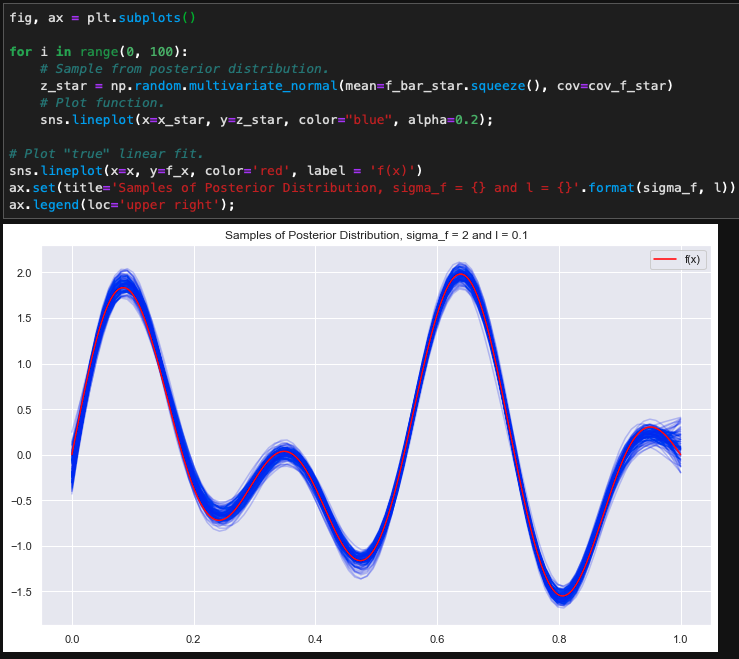
\includegraphics[scale=0.32]{images/code_sample_posterior_example2.png} 
\caption{We sample from the posterior space of functions by plotting their realization on $n_*=100$ points. }
\end{figure}
\end{center}
\end{frame}


\begin{frame}{Hyperparameter Estimation}{\cite[Chapter 2.3, 5]{RW05}}
\begin{center}
\begin{figure}
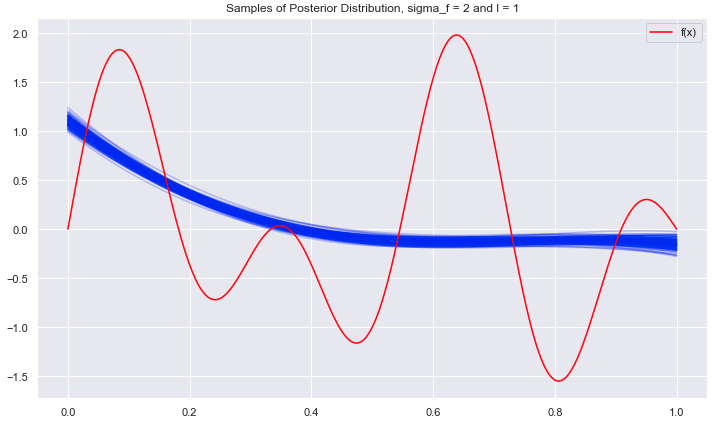
\includegraphics[scale=0.21]{images/hyp_posterior_1_example2}
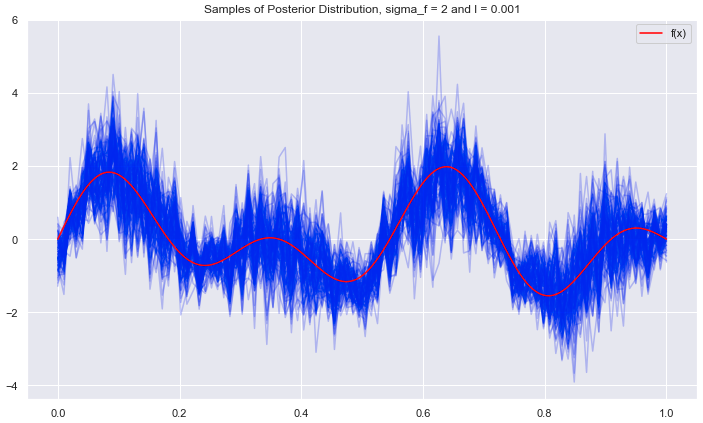
\includegraphics[scale=0.21]{images/hyp_posterior_2_example2}
\caption{Samples from two gaussian processes with different scale parameters (left: $\ell=1$ and right: $\ell = 0.001$).}
\end{figure}
\end{center}
\begin{block}{Methods}
\begin{itemize}
\item Marginal Likelihood ($\theta$ = parameter vector)
\begin{align*}
\log(p(y|X, \theta)) = -\frac{1}{2}y^T (K+\sigma_n^2I)^{-1}y - \frac{1}{2}\log|K+\sigma_n^2I| - \frac{n}{2}\log (2\pi)
\end{align*}
\item Cross Validation
\end{itemize}
\end{block}
\end{frame}

\section{The Kernel Space}

\begin{frame}{The Kernel Space}{\cite{ROERGA}, \cite[Chapter 4]{RW05}}
Let $k_1, k_2: \mathcal{X}\times\mathcal{X}\longrightarrow \mathbb{R}$ be two kernels, then the following are also kernels 
\begin{itemize}
\item $k_1 + k_2$ 
\item $k_1 \times k_2$
\item $k_1*k_2$ (convolution)
\end{itemize}
If $k: \mathcal{X}_1\times\mathcal{X}_1\longrightarrow \mathbb{R}$ and $h: \mathcal{X}_2\times\mathcal{X}_2\longrightarrow \mathbb{R}$ are two kernels, then the following are also kernels (on $\mathcal{X}_1 \times \mathcal{X}_2$)
\begin{itemize}
\item $k_1 \oplus k_2$ 
\item $k_1 \otimes k_2$
\end{itemize}
\begin{block}{Remark (\cite[Chapter 4.3]{RW05})}
There is a rich theory of spectral theory for kernels by considering the integral operator $T_k : L^2(\mathcal{X}, \mu) \longrightarrow L^2(\mathcal{X}, \mu)$ (where $(\mathcal{X}, \mu)$ is a finite measure space and $k\in L^{\infty}(\mathcal{X}\times \mathcal{X} , \mu\times\mu)$). 
\begin{align*}
(T_k\phi)(x) = \int_{\mathcal{X}} k(x, x')\phi(x') d\mu(x')
\end{align*}
\end{block}
\end{frame}

\section{Example: Time Series}

\begin{frame}{Example: Periodic Component I (\cite{gaussian_process_time_series_2019})}{\cite[Section 1.7. Gaussian Processes]{scikitlearn}}
\begin{center}
\begin{figure}
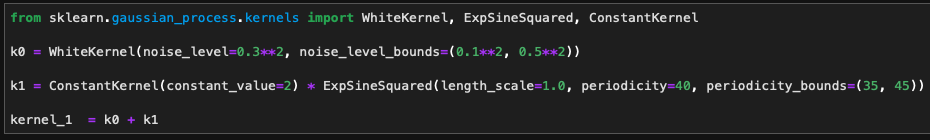
\includegraphics[scale=0.3]{images/code_kernel_1_example3.png}
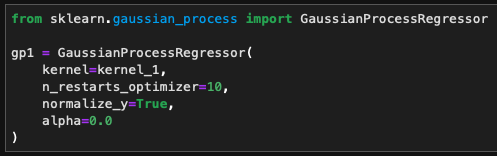
\includegraphics[scale=0.3]{images/gp1_example3.png}
\end{figure}
\end{center}
\begin{center}
\begin{figure}
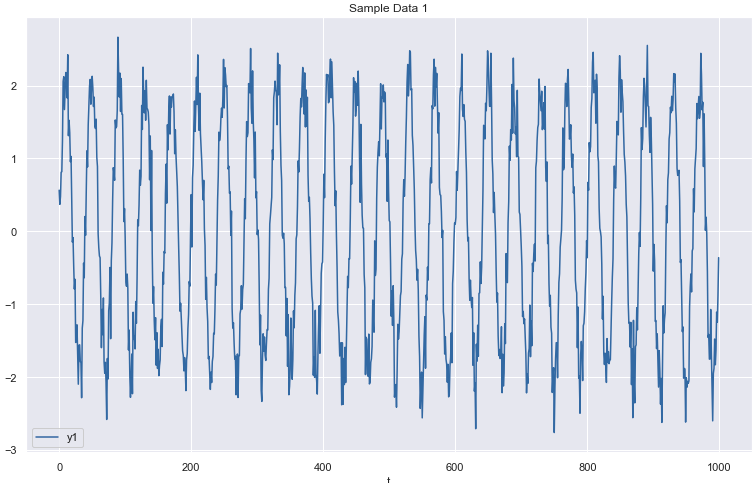
\includegraphics[scale=0.20]{images/sample_1_example3.png}
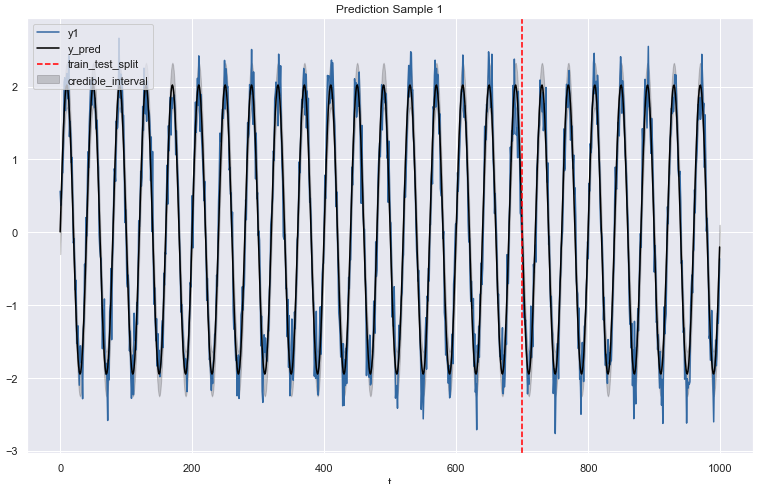
\includegraphics[scale=0.20]{images/pred_1_example3.png}
\end{figure}
\end{center}
\end{frame}

\begin{frame}{Example: Add Linear Trend }
\begin{center}
\begin{figure}
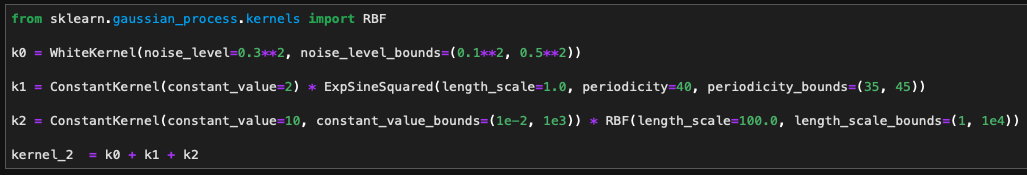
\includegraphics[scale=0.3]{images/code_kernel_2_example3.png}
\end{figure}
\end{center}
\begin{center}
\begin{figure}
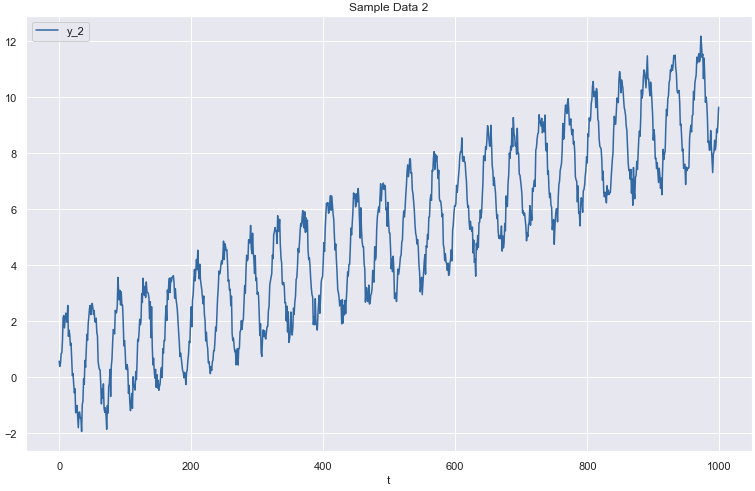
\includegraphics[scale=0.20]{images/sample_2_example3.png}
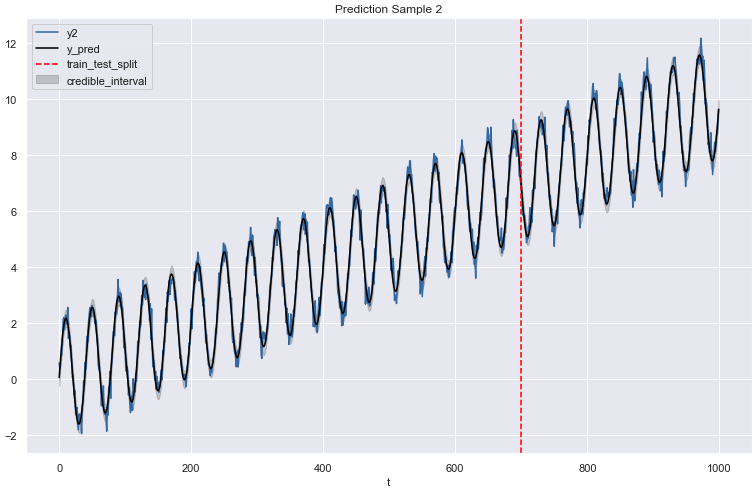
\includegraphics[scale=0.20]{images/pred_2_example3.png}
\end{figure}
\end{center}
\end{frame}


\begin{frame}{Example: Add Periodic Component II }
\begin{center}
\begin{figure}
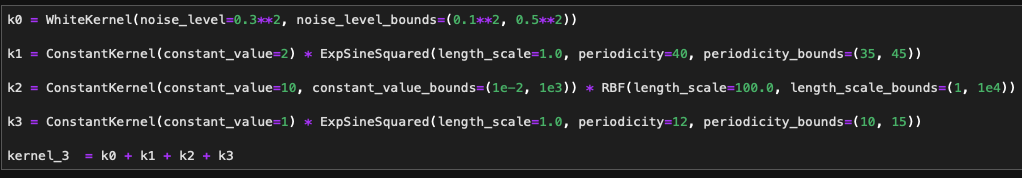
\includegraphics[scale=0.3]{images/code_kernel_3_example3.png}
\end{figure}
\end{center}
\begin{center}
\begin{figure}
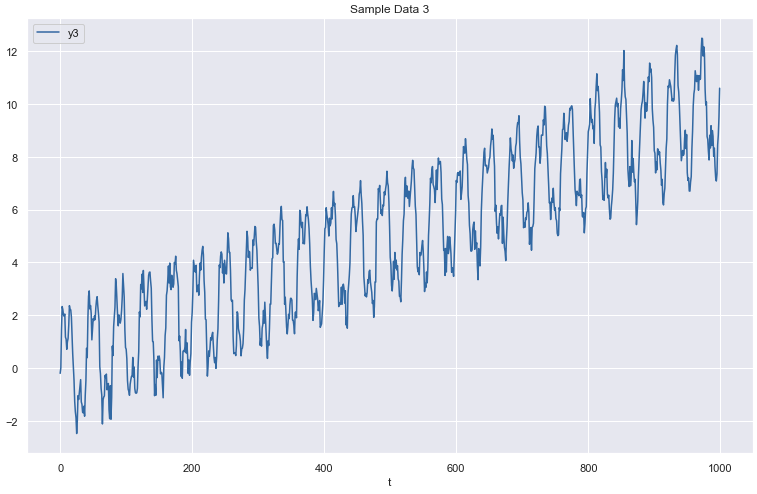
\includegraphics[scale=0.20]{images/sample_3_example3.png}
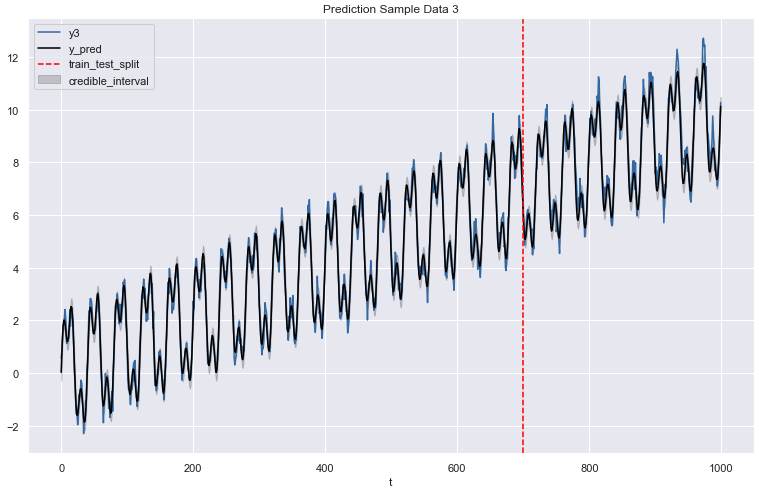
\includegraphics[scale=0.20]{images/pred_3_example3.png}
\end{figure}
\end{center}
\end{frame}

\begin{frame}{Computational Challenges}
\begin{itemize}
\item Calculating the posterior mean and covariance matrix requires $\mathcal{O}(n^3)$ computations. 
\item A practical implementation of Gaussian process regression is described in \cite[Algorithm 2.1]{RW05}, where the Cholesky decomposition is used instead of inverting the matrices directly. 
\item There are remarkable approximation methods for Gaussian processes to speed up the computation (\cite[Chapter 20.1]{BDA13})
\end{itemize}
\end{frame}



\begin{frame}[t, allowframebreaks]
\frametitle{References}
\footnotesize{
\setbeamertemplate{bibliography item}[text]
\bibliographystyle{plain}
\bibliography{references} 
}
\end{frame}

\begin{frame}
\begin{center}
\huge{Thank You!}%\footnote{Especially to all the organizers and speakers!}
\end{center}

\begin{block}{Contact}
\begin{itemize}
\item \faRocket $\:$ \href{https://juanitorduz.github.io}{https://juanitorduz.github.io}
\item \faGithub $\:$ \href{https://github.com/juanitorduz}{github.com/juanitorduz}
\item \faTwitter $\:$ \href{https://twitter.com/juanitorduz}{juanitorduz}
\item \faEnvelope $\:$ \href{mailto:juanitorduz@gmail.com}{juanitorduz@gmail.com}
\end{itemize}
\end{block}

\end{frame}

\end{document}





























